\chapter{Proposed Method and Experiments}
\label{chap:experiment}
\thispagestyle{empty}
In this chapter, we will propose a diffusion-based pipeline for watermark removal. We will then focus on conducting experiments using the proposed pipeline for watermark removal, as detailed in Section \ref{sec:pipeline}. The experiments utilize the ImageNet dataset, with the Pokémon dataset serving as the watermark. Further information about the datasets will be provided in Section \ref{sec:dataset}. The results of our pipeline, from watermark embedding to removal and image inpainting, will be presented step by step. Section \ref{sec:removal} will discuss the outcomes in detail.

Upon completing all experiments, we aim to establish metrics for evaluation. Section \ref{sec:metrics} will provide a comprehensive discussion on these metrics, offering an overview and assisting in selecting the most suitable metric to assess the effectiveness of our pipeline in watermark removal.
% Summary experiments:
% proposed pipeline done + result + masks position
% datasets
% metrics

\section{Proposed Watermark Attacking Pipeline}
\label{sec:pipeline}
As backgrounds and methodologies relevant to the Watermark Attacking problem have been clarified, in this section we introduce our proposed pipeline designed to address this challenge. Figure \ref{figure:overall_pipeline} provides an overview of our comprehensive pipeline, encompassing the following steps
\begin{enumerate}
 \item The original image undergoes Watermark Embedding through the Watermark Embedder. The watermark information for each image is also stored for later evaluation.
 \item The watermarked image then passes through a Watermark Localization model, revealing regional information of the watermark. The watermark is then masked from the image, creating a degraded image to be inpainted.
 \item Finally, the inpainting process, specifically I$^2$SB in our case, reconstructs the image to closely resemble the original image.
\end{enumerate}
\begin{figure}[t]
 \centering
 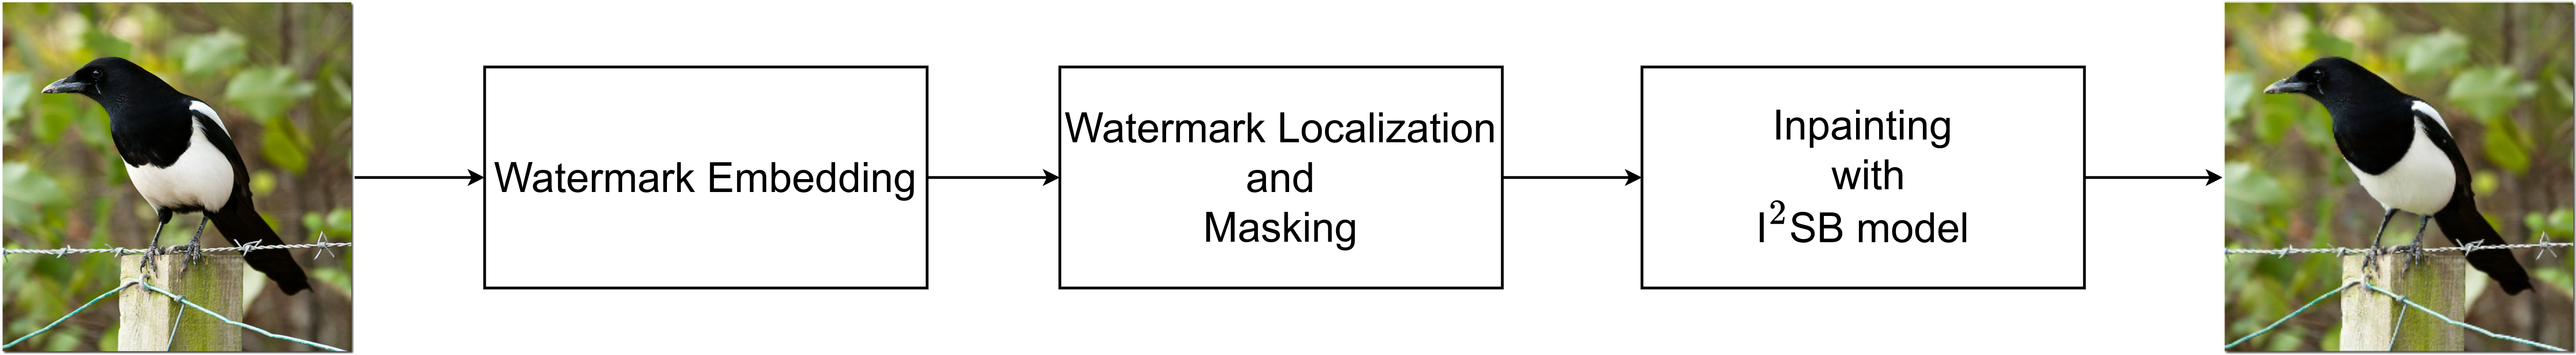
\includegraphics[width = \textwidth]{img/overall.png}
 %\vspace{0.5cm}
 \caption{Overall pipeline for Watermark Attacking}
 \label{figure:overall_pipeline}
\end{figure}

% \begin{figure}[t]
%     \centering
%     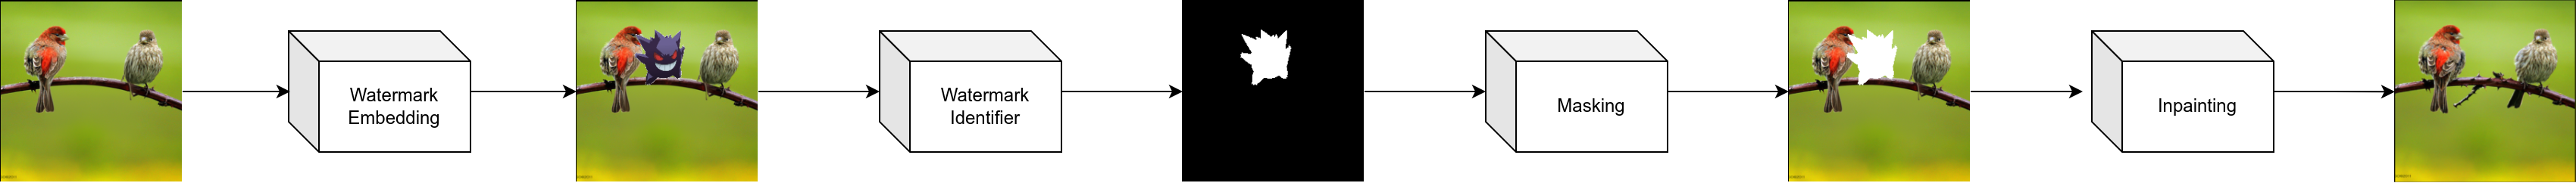
\includegraphics[width = \textwidth]{img/pipeline1.png}
%     
%     \caption{Approach 1}
%     \label{figure:appr1}
% \end{figure}

% \begin{figure}[t]
%     \centering
%     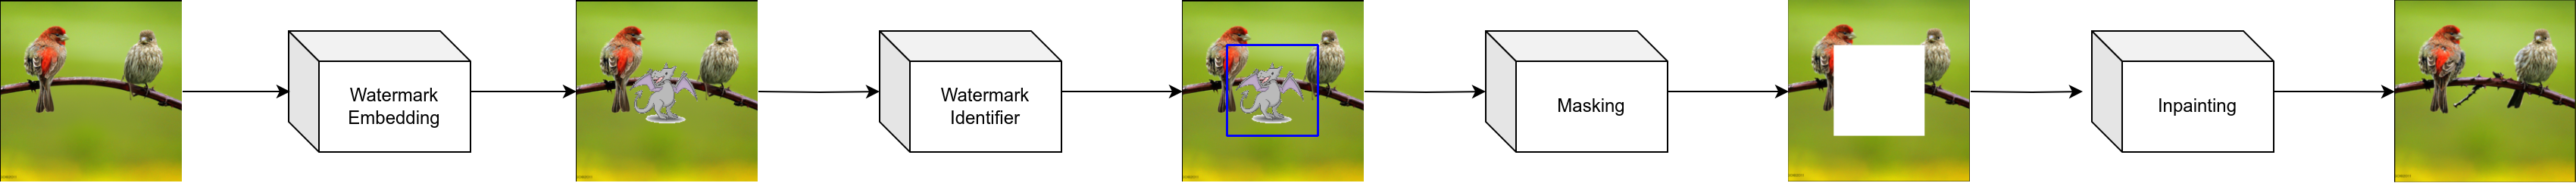
\includegraphics[width = \textwidth]{img/pipeline2.png}
%     
%     \caption{Approach 2}
%     \label{figure:appr2}
% \end{figure}
\subsection{Watermark Embedding}
\label{chapter:d:section:emb}
To begin, we will generate a watermarked dataset by embedding the watermark into the original images. Algorithm \ref{algorithm:embed} provides an overview of the watermark embedding process that we have implemented.
\begin{figure}[t]
    \centering
    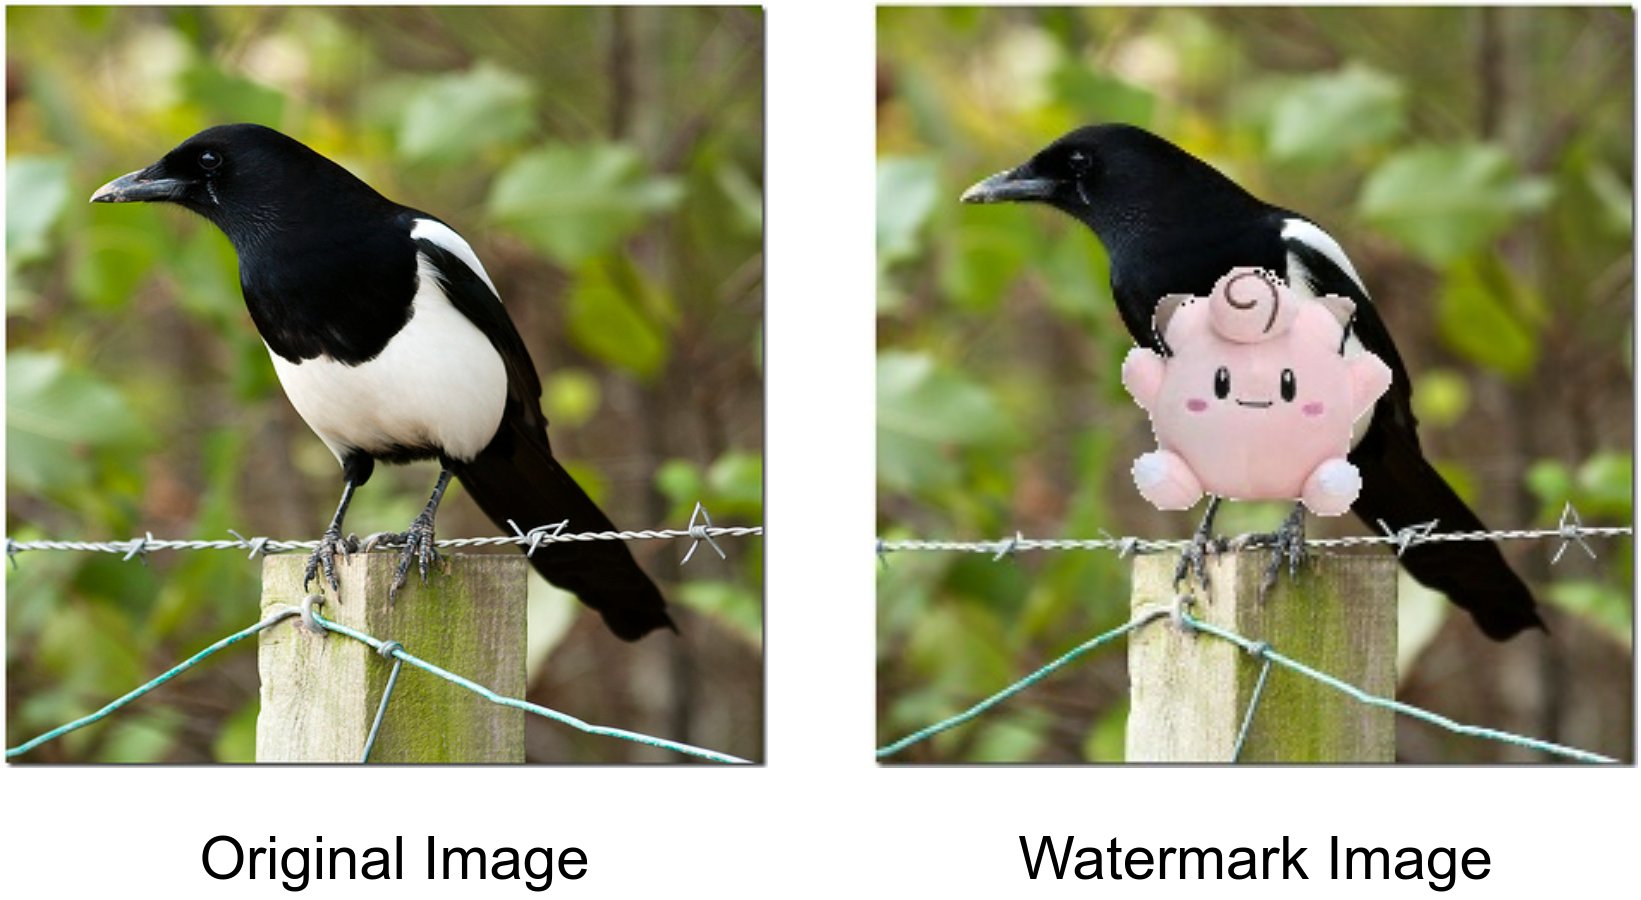
\includegraphics[width=0.75\linewidth]{img/embedded.png}
    %\vspace{0.5cm}
    \caption{Embed a watermark into the image}
    \label{figure:embed_img}
\end{figure}
To embed the watermark, we begin with two datasets: one containing base images and the other comprising watermark images. For each image in the base dataset, we randomly select a watermark, extract its foreground using image processing, and extract the background by a specified color. For this step to be successful, it is crucial to choose a watermark dataset with minimal background detail.

The foreground of the watermark image is then placed onto the base image at a specified location, which can be either random or at the center of the image. After embedding the watermark, we save the watermarked image along with location information, such as bounding box or label map, for future reference. The resulting watermarked image is illustrated in Figure \ref{figure:embed_img}.
\begin{algorithm}[t]
 \caption{Embedding}
 \label{algorithm:embed}
 \begin{algorithmic}[1]
  \STATE {\bfseries Input:} clean dataset $A$ and watermark dataset $B$
  \FOR{$image$ {\bfseries in} $A$}
  \STATE Get random $sample$ from $B$
  \STATE Extract $foreground$ from $sample$
  \STATE Get $location$ to place watermark
  \STATE Place the $foreground$ on $location$ of $image$, save to $processed$
  \STATE Append $processed$ image to embedded dataset $C$
  \ENDFOR
  \STATE {\bfseries return} $C$
 \end{algorithmic}
\end{algorithm}
\subsection{Watermark Localization}
After embedding and obtaining the watermarked dataset, the next step involves identifying its location information and subsequently masking it for the image inpainting task. Regarding the identifier, we consider two approaches: Image Segmentation and Object Detection.
\subsubsection{Image Segmentation Approach}
In this approach, we aim to construct the watermark identifier as an object detection model. The pipeline for this approach is illustrated in Figure \ref{figure:segmentation}. There are various techniques for performing image segmentation, such as thresholding, clustering, region-based, edge-based, and graph-based methods. With the development of deep learning, many neural network architectures have been proposed for image segmentation tasks, such as U-Net, FastFCN \cite{wu2019fastfcn}, Gated-SCNN \cite{takikawa2019gated}, and others. These architectures usually consist of an encoder and a decoder, where the encoder extracts features from the image and the decoder generates the segmentation mask. Some architectures also use additional modules or components, such as skip connections, attention mechanisms, or pyramid up-sampling, to improve the performance and accuracy of the segmentation
\begin{figure}[t]
 \centering
 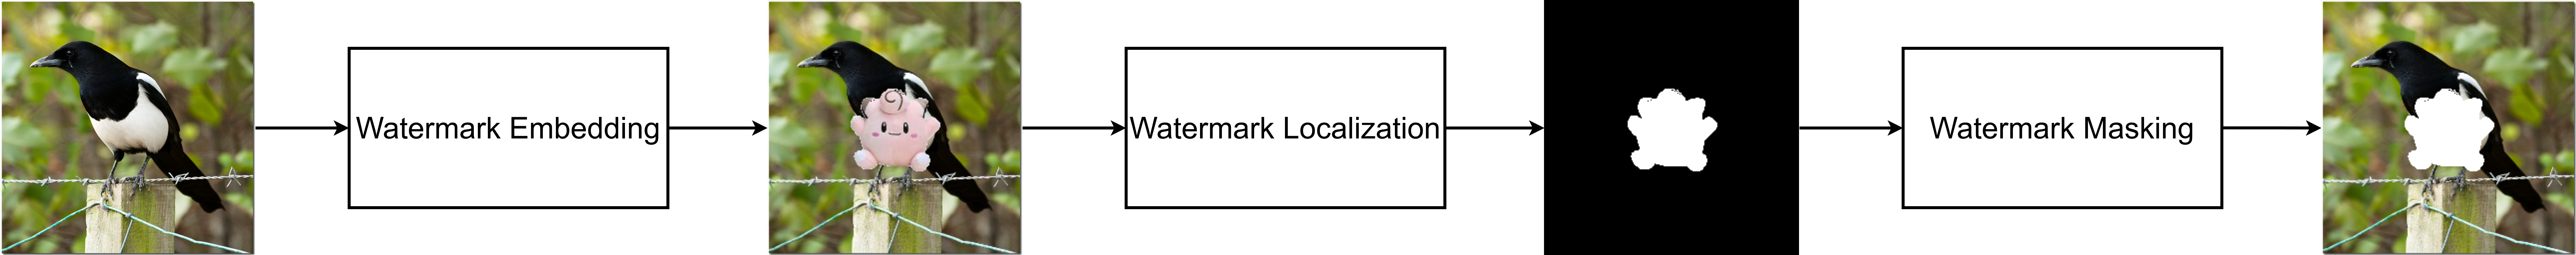
\includegraphics[width=\linewidth]{img/segmentation.png}
 %\vspace{0.5cm}
 \caption{Identify the watermark in image with Image Segmentation Approach}
 \label{figure:segmentation}
\end{figure}

The output of the image segmentation model is a segmentation map, with will extract the watermark out of the original image, as shown in the third image from left to right in Figure \ref{figure:segmentation}. The output from the segmentation approach provides a well-fitted segmentation for the watermark, ensuring that the mask precisely erases only the watermark during inpainting. This approach helps conserve the areas requiring inpainting, particularly those with intricate details. However, relying on segmentation introduces a strong dependency on the accuracy of the segmentation map. If the segmentation inaccurately fits the watermark, it may miss certain details, impacting the quality of the image after removing the watermark. Additionally, extending the segmentation map can be challenging, making it difficult to use the output if the watermark localization is incorrect.
\subsubsection{Object Detection Approach}
In this approach, we aim to construct the watermark identifier as an object detection model. The pipeline for this approach is illustrated in Figure \ref{figure:detection}. Object detection is a fundamental task in computer vision that aims to locate and classify objects in an image. Object detection methods can be broadly categorized into two types: two-stage detectors and one-stage detectors. Two-stage detectors first generate a set of region proposals that may contain objects, and then apply a classifier and a regressor to refine the proposals and predict the object labels and bounding boxes. One-stage detectors directly predict the object labels and bounding boxes for all the pixels or anchors in the image, without using region proposals.

Two-stage detectors are usually more accurate than one-stage detectors, but also slower and more complex. The most representative two-stage detector is the R-CNN family, which includes R-CNN \cite{girshick2014rich}, Fast R-CNN \cite{girshick2015fast}, and Faster R-CNN  \cite{ren2016faster}. R-CNN extracts features from each region proposal using a convolutional neural network (CNN), and then uses a support vector machine (SVM) and a linear regressor to classify and localize the objects. Fast R-CNN improves R-CNN by sharing the CNN features among all the region proposals, and using a softmax classifier and a bounding box regressor instead of SVM and linear regressor. Faster R-CNN further improves Fast R-CNN by replacing the selective search algorithm for generating region proposals with a region proposal network (RPN), which is a fully convolutional network that can be trained end-to-end with the detection network.

One-stage detectors are usually faster than two-stage detectors, but also less accurate and more prone to false positives. The most representative one-stage detector is the YOLO \cite{redmon2016you} family, which now release up to YOLOv8. YOLO divides the input image into a grid of cells, and predicts the object labels and bounding boxes for each cell.

Moreover, some recent object detection methods try to bridge the gap between two-stage and one-stage detectors, by combining the advantages of both types. For example, RetinaNet \cite{lin2017focal} is a one-stage detector that introduces a focal loss function to address the class imbalance problem, which is the main cause of the lower accuracy of one-stage detectors. DERT \cite{carion2020end} is a two-stage detector that uses a dynamic and efficient region transformer to generate adaptive region proposals, which can reduce the computation and memory cost of the detection network.
\begin{figure}[t]
 \centering
 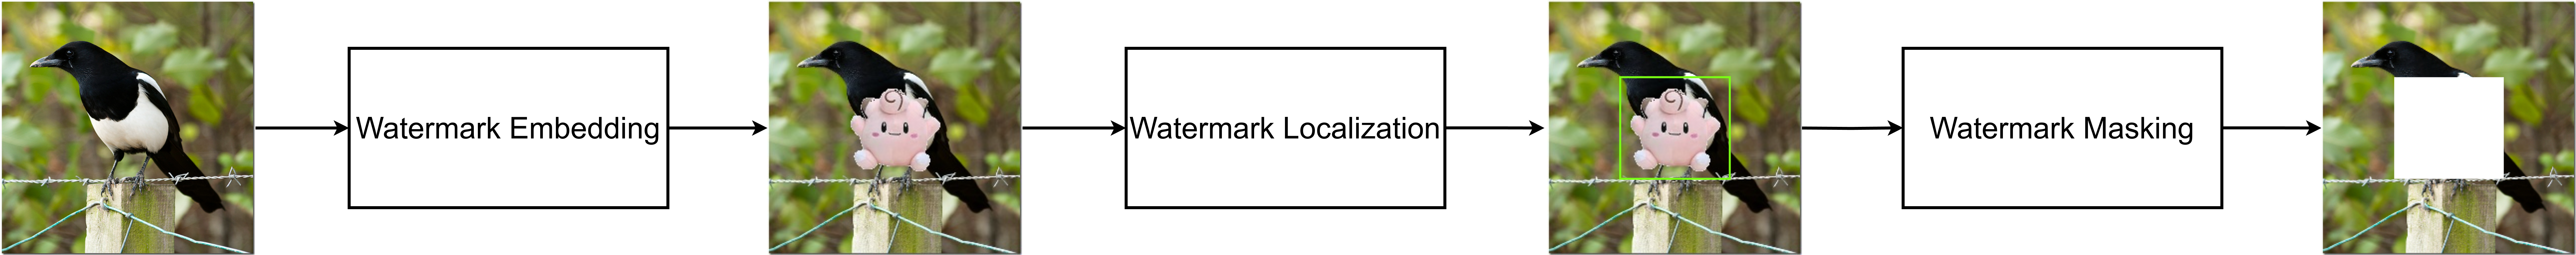
\includegraphics[width=\linewidth]{img/detection.png}
 % %\vspace{0.5cm}

 \caption{Identify the watermark in image with Object Detection Approach}
 \label{figure:detection}
\end{figure}

The output of the object detection model is a bounding box, indicating the rectangular area where the watermark is located. Consequently, the masking area, once the box is determined, may be larger than the watermark itself. This can result in the inpainting task having to restore a larger masked area compared to the segmentation approach. However, with the location provided by the bounding box, the model's error rate may be lower than that of segmentation. This is because the segmentation approach needs to predict the exact structure of the watermark, which could be prone to missing some details.

Moreover, with the bounding box, we have the flexibility to add a padding size to the box if needed. On the contrary, extending the segmentation map can be challenging. In summary, the object detection approach makes it easier to accurately detect the location of the watermark, but the larger bounding box may pose challenges for the inpainting task.

% In summary of this section, within the scope of this project, we have not yet developed a watermark identifier due to time constraints. Consequently, to execute this pipeline, we leverage the saved watermark labeling information, as discussed in Section \ref{chapter:d:section:emb}. This information is utilized for masking, enabling us to proceed directly to the image inpainting task. The development of the watermark identifier will be continued in the next phase of this project.
\subsection{Image Inpainting}
Finally, after obtaining a masked image by applying the detected watermark mask, we proceed with the inpainting task. For this task, we employ the I$^2$SB model to inpaint the masked region in the image. The process is illustrated in Figure \ref{figure:inpainting_arch}.
\begin{figure}[t]
 \centering
 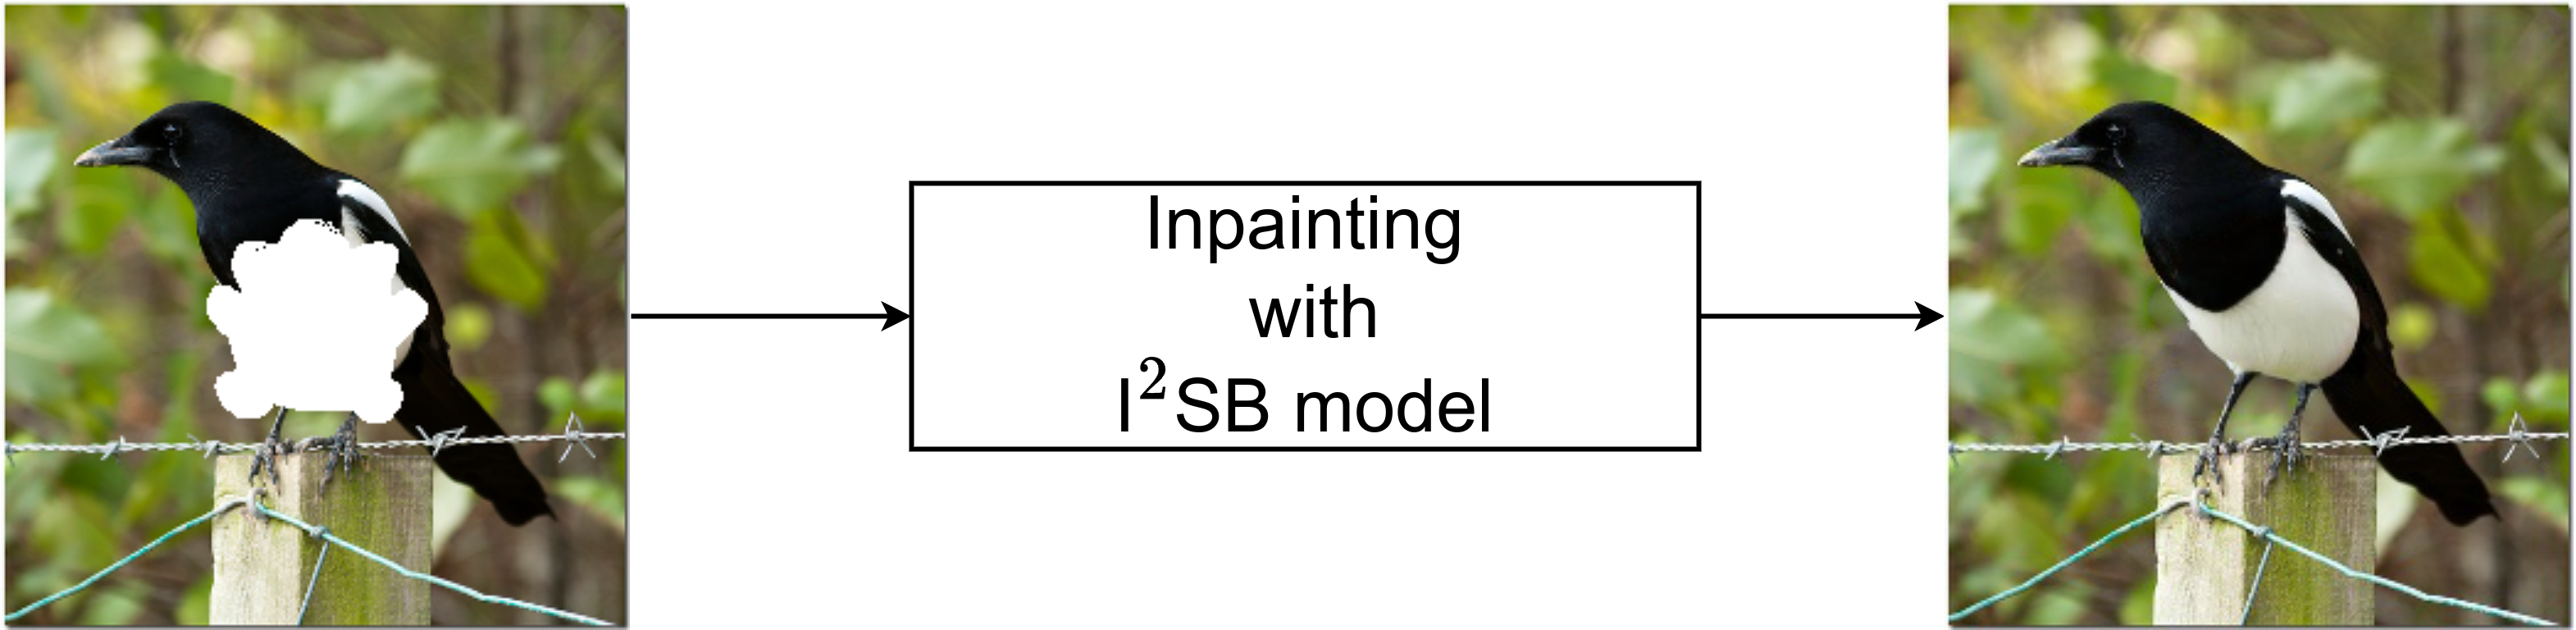
\includegraphics[width=0.75\linewidth]{img/inpainting_arch.png}
 %\vspace{0.5cm}

 \caption{Inpainting the mask image with I$^2$SB}
 \label{figure:inpainting_arch}
\end{figure}
The process of inpainting is explained in Figure \ref{figure:inpainting_arch}. We work with a set of details that include both the original and the covered-up image. From this information, we pick out the part of the image that is covered. The aim of this inpainting task is to bring back the covered section we have identified, hoping to recreate an image that closely resembles the original one.

\section{Datasets}
\label{sec:dataset}
\subsection{Image Dataset}
\label{sec:dataset:clean}

We start conducting the experiments on our pipeline by choosing a dataset as the starting point for our work, where we will add watermarks and later remove them. Since we are planning to use the I$^2$SB model, and reproducing the training on other datasets is a bit tricky due to limited resources, we decide to go with a dataset where the model has already been trained. The I$^2$SB model is primarily trained on ImageNet with an image size of $256 \times 256$ for the task of image inpainting. Therefore, we will be using ImageNet as our primary dataset for the upcoming experiments. Additionally, we will carry out experiments in the image inpainting task using the ImageNet 10k validation subset, which comprises approximately 10,000 samples.

\subsection{Watermark Dataset}
\label{sec:dataset:wtm}
For the watermark dataset, we choose a dataset with minimal background detail. Therefore, we choose a dataset we discovered on Kaggle named \textit{Pokémon from First Gen}\footnote{\href{https://www.kaggle.com/datasets/unexpectedscepticism/11945-pokemon-from-first-gen}{Pokemon from First Gen Dataset, Kaggle}}. This dataset comprises approximately 12,000 samples of Pokémon characters, all featuring a white or transparent background. This simplicity makes it easier for us to embed these characters into the original images. You can view samples from this dataset in Figure \ref{fig:Pokemon}.

\begin{figure}[t]
    \centering
    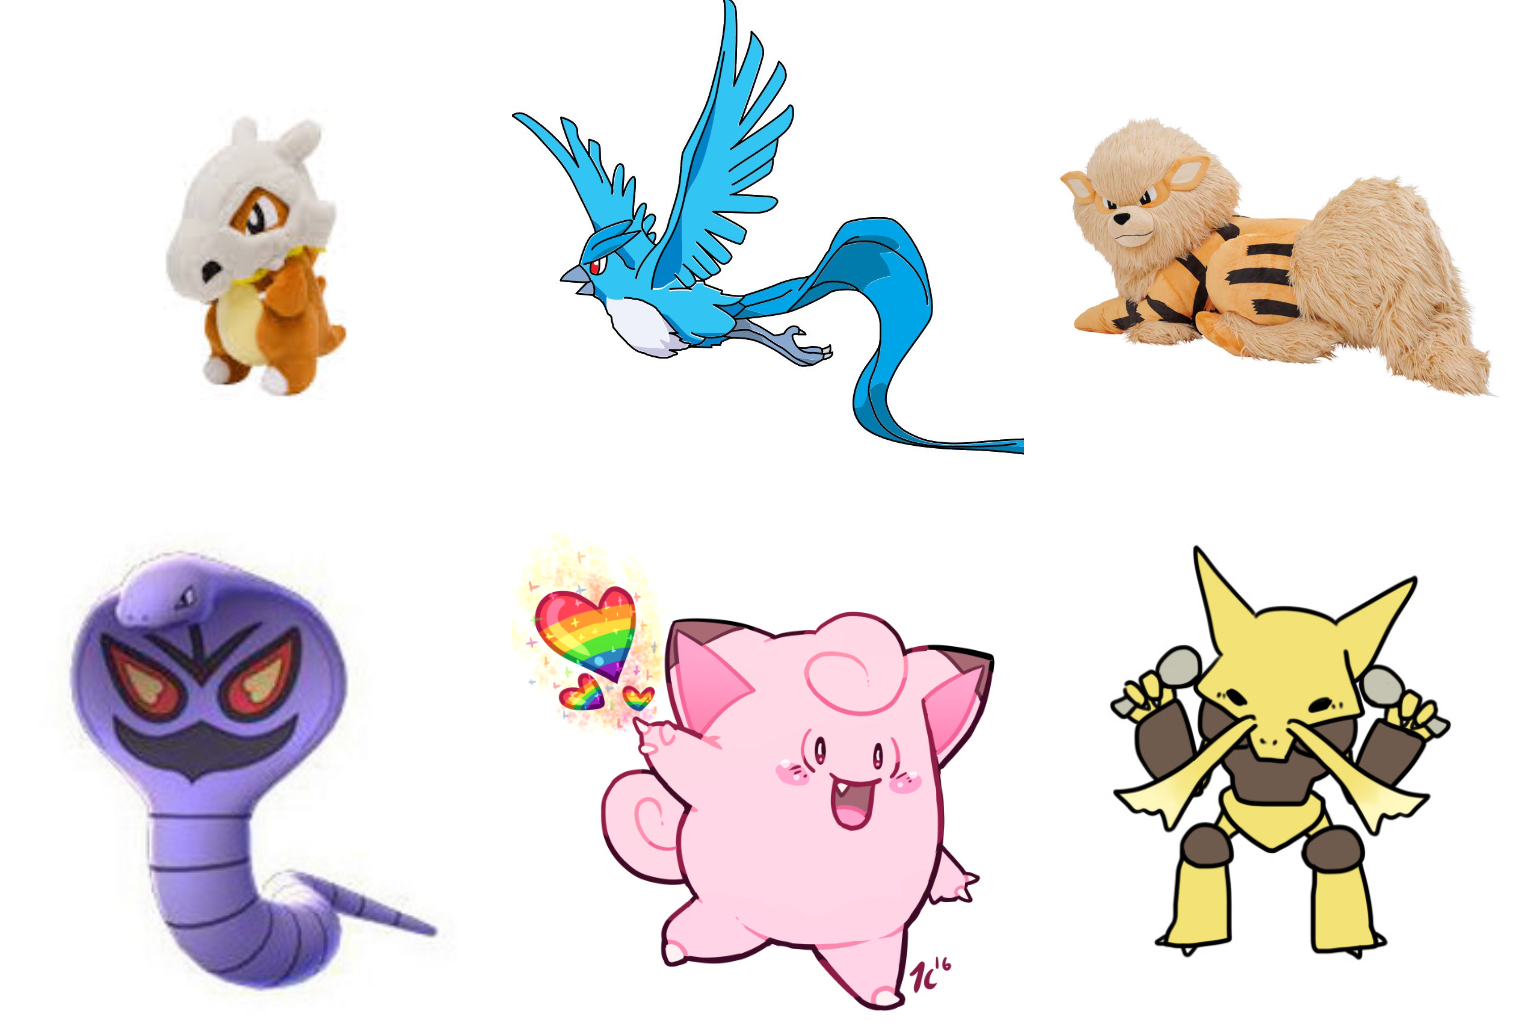
\includegraphics[width = 0.5 \textwidth]{img/Pokemon.png}
    %\vspace{0.5cm}
    \caption{Watermark Dataset}
    \label{fig:Pokemon}
\end{figure}

\subsection{Embedded Watermark Image}
% \textcolor{red}{Move to dataset for watermarked image dataset}
\label{sec:ewi}
\label{sec:embedding}
In this section, we will conduct experiments on embedding the watermarks into images. Our goal is to create a dataset of watermarked images that can later be used to attack the watermark. We performed watermark embedding on the ImageNet dataset as mentioned in Section \ref{sec:dataset:clean}. Samples of this dataset are illustrated in the first row of Figure \ref{fig:watermark-embedding}.

\begin{figure}[t]
    \centering
    \includegraphics[width=0.8\linewidth]{img/watermark-embedding.png}
    \caption{Watermark embedding and its positional information}
    \label{fig:watermark-embedding}
\end{figure}

To embed the watermark, we need a watermark dataset as mentioned in Section \ref{sec:dataset:wtm}. The watermark images we choose have a white background, making it easier to separate the object from the background using image processing techniques. Since image pixels are represented by values ranging from 1 to 255, the white background has a value of 255 across all its channels (RGB). We create a mask by assigning a value of 1 to pixels that differ from 255, and a value of 0 to pixels with the value of 255. This mask effectively isolates the watermark object from its background, making it ready to be embedded into the target image. The Figure \ref{fig:wtm-obj-mask-1} illustrates the watermark image and its corresponding mask, which labels the watermark object.

\begin{figure}[t]
    \centering
    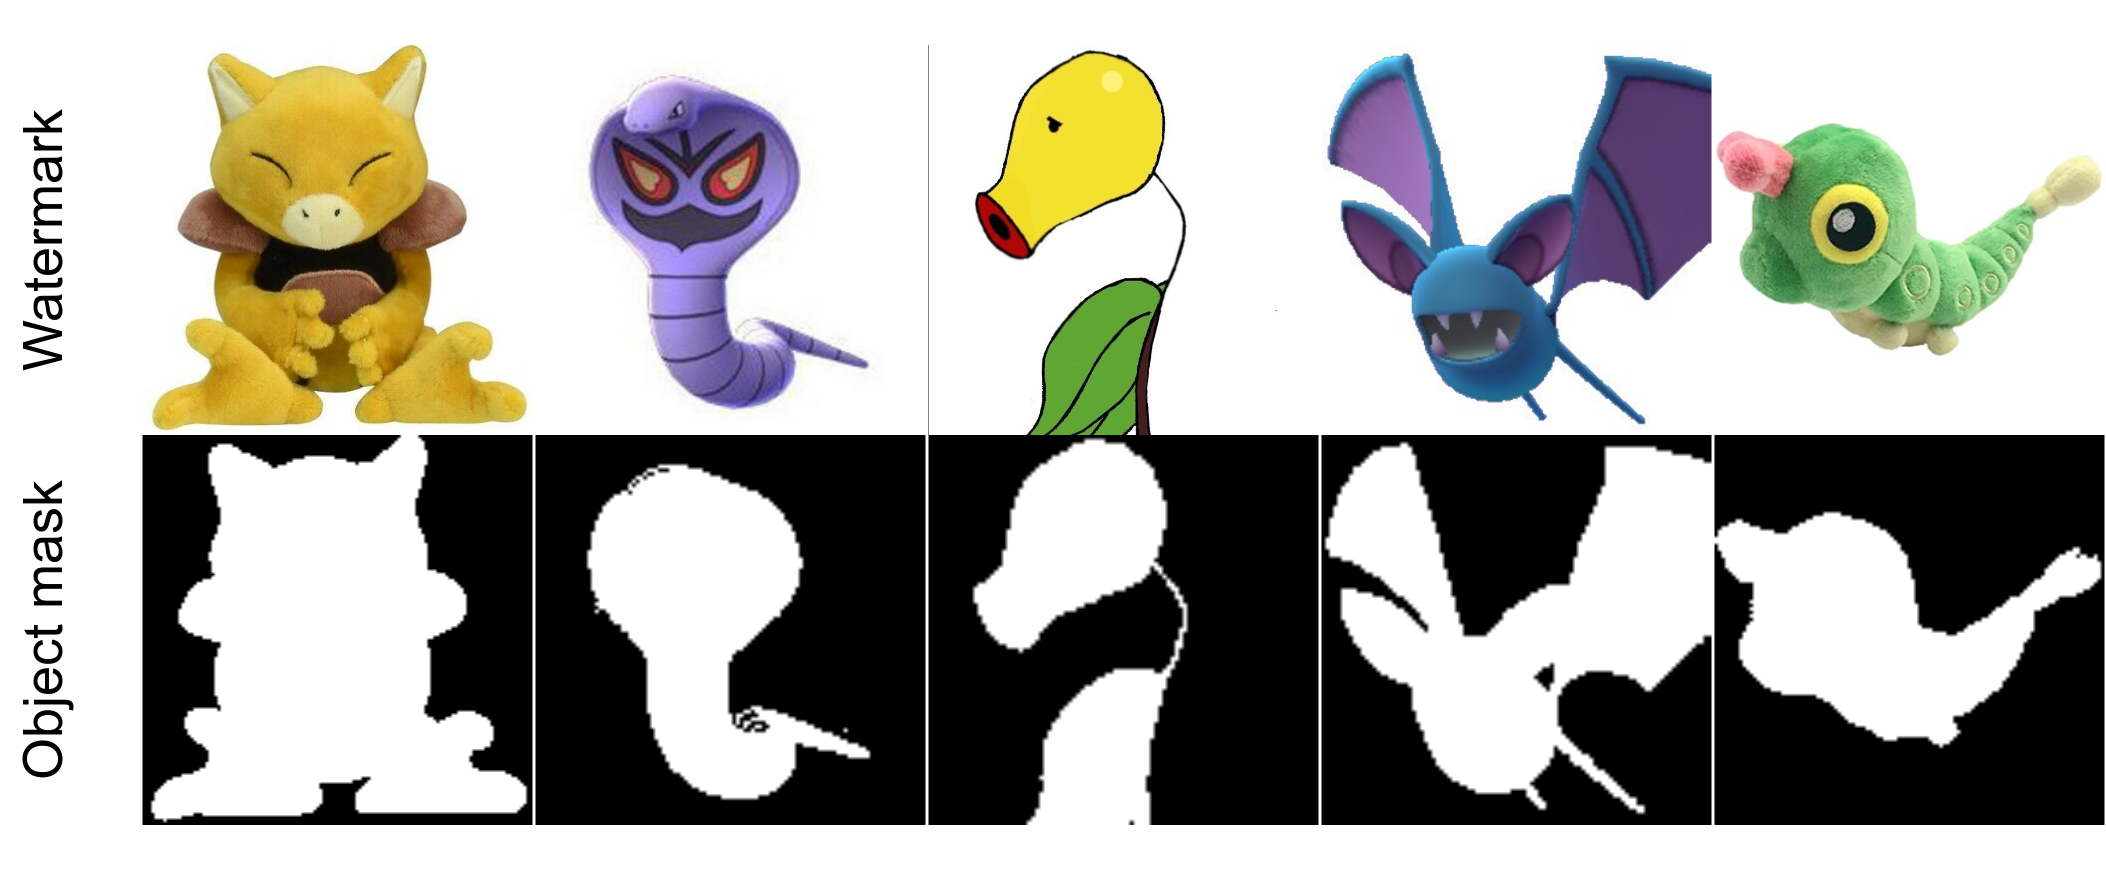
\includegraphics[width=0.8\linewidth]{img/watermark-and-objectmask.png}
    %\vspace{0.5cm}
    \caption{Watermark image and its object mask}
    \label{fig:wtm-obj-mask-1}
\end{figure}

Sometimes, however, the watermark object itself has pixel values of 255 across all its channels (RGB), causing the mask to fail, as shown in the first and second row of Figure \ref{fig:wtm-with-white-detail}. To handle this case, we need to use a morphological image processing method called Closing. This method will connect the black holes in the object mask and ensure that the white areas within the object are included in the mask, as shown in the last row of Figure \ref{fig:wtm-with-white-detail}.

\begin{figure}[t]
    \centering
    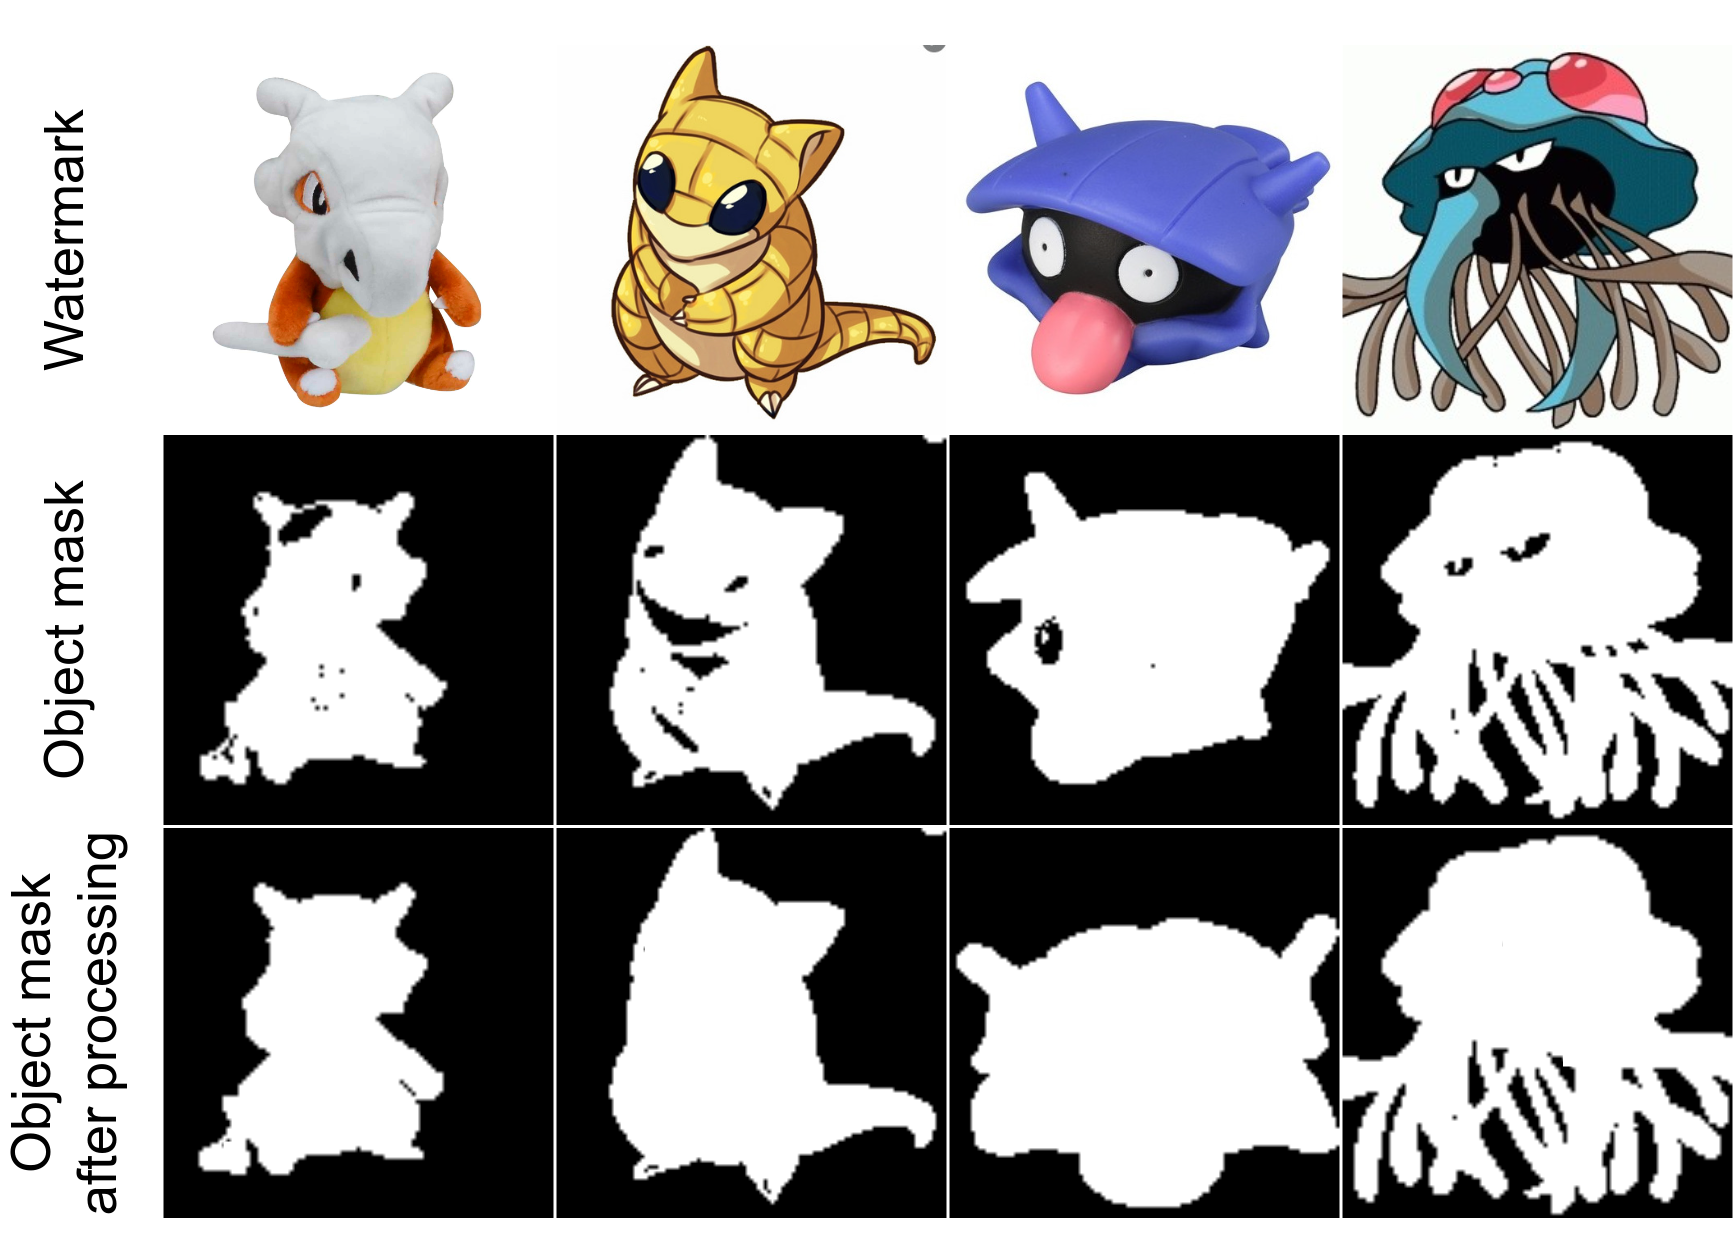
\includegraphics[width=0.8\linewidth]{img/wtm_embed_processing.png}
    %\vspace{0.5cm}
    \caption[Watermark image morphological image processing methods]{Watermark image that its object have white detail and its post-processing by using morphological image processing methods}
    \label{fig:wtm-with-white-detail}
\end{figure}

In addition, some images in the watermark dataset have transparency, which includes a fourth channel for opacity. These images indicate the opacity of the watermark object with a value of 1, meaning fully visible, and the background with a value of 0, meaning fully invisible. In this case, we can separate the watermark object from its background by creating a mask that matches the values of the opacity channel. Then, we reduce these watermark images to the usual three channels (RGB) for convenience in processing.

The watermark object now is ready to embed, we then choose a location in the original image to place the watermark. This is done by selecting a point that marks where the top-left corner of the watermark image will be positioned on the original image. After that, we paste the entire watermark image, ensuring that the top-left corner aligns with the chosen point. The size of the watermark image will be constrained to cover 10-30\% of the original image area. Additionally, we adjust the opacity of the watermark to vary from 0.5 to 1. This adjustment is achieved through an interpolation of pixel values between the original image and the watermark image. This ensures that the watermark not only overlays the content of the original image but also blends into the image, sometimes becoming partially transparent. The result of watermark embedding will be shown in the second row of Figure \ref{fig:watermark-embedding}.

Finally, after embedding the watermark, we save the watermarked image along with its watermark mask and bounding box. This information proves valuable for subsequent steps, particularly in providing ground-truth data for the watermark localization task. These information will be bounding box or object mask as shown in the third and last row of Figure \ref{fig:watermark-embedding}.

\section{Metrics}
\label{sec:metrics}
In this section, our aim is to identify suitable metrics for evaluating our pipeline. Considering that we are implementing two tasks: image inpainting, a type of image-to-image method, and watermark localization using Semantic Segmentation, we will focus on evaluating metrics commonly used in these domains. These metrics will serve as the basis for evaluating our work in the following section.

\subsection{Peak Signal-to-Noise Ratio}

The PSNR block computes the peak signal-to-noise ratio, in decibels, between two images. This ratio is used as a quality measurement between the original and a reconstructed image. The higher the PSNR, the better the quality of the reconstructed image. The Mean-Squared Error (MSE) and the peak signal-to-noise ratio (PSNR) are used to compare image compression quality. The MSE represents the cumulative squared error between the compressed and the original image, whereas PSNR represents a measure of the peak error. The lower the value of MSE, the lower the error.

To compute the PSNR for two $m \times n$ images, the block first calculates the Mean-Squared Error using the following equation
\begin{equation}
    \text{MSE} = \dfrac{1}{mn}\sum\limits_{p}[I(p)-\hat{I}(p)]^2,
\end{equation}
where $I$ is target, $\hat{I}$ is predicted image and $p$ is the respective pixel in each image. Then the block computes the PSNR using the following equation

\begin{equation}
    \text{PSNR} = 10\log_{10}\left(\dfrac{\text{MAX}_\text{I}^2}{\text{MSE}}\right).
\end{equation}
where $\text{MAX}_\text{I}$ is the maximum fluctuation in the input image data type. For example, if the input image has a double-precision floating-point data type, then $\text{MAX}_\text{I}$ is 1. If it has an 8-bit unsigned integer data type, $\text{MAX}_\text{I}$ is 255 and so on. This metric attempts to compare the pixel-to-pixel correspondence between the original image and the reconstructed one. Consequently, it may prove to be sensitive in the context of image inpainting tasks, particularly when reconstructing images with intricate details that are masked.

In this metric, we aim to calculate the ratio of peak signal to the noise instead of only focusing on the noise, as done in Mean-Squared Error. This is because noise can have various ranges, such as 0-255 for an 8-bit image or 0.0-1.0 for a floating-point image type. Simply comparing errors is not sufficient for comparing across different tasks and reporting results accurately. Therefore, we need to normalize the metric to provide a more generalized measure by dividing the peak signal to its noise, enabling more precise comparisons across different types of images or signals.



% \textcolor{red}{-> p where p is per pixel in the image\\
%     -> $I$ is target and $\hat{I}$ is predicted image\\
%     -> we calculate the ratio of Peak signal to the noise instead of focus only on the noise because the noise have a various range (such as in image we have ranges of 0-255 if it is an 8-bit image and 0.0-1.0 if it is a floating-point image type) and we need a step to re-scale in a general metric\\
%     -> The logarithm in the formula is the value of dB in signal measure. It may be used to scale the small or large value into an acceptable value\\
%     -> Name of the metric in formula should be wrapped in text\{\}}

% \subsection{Classification Accuracy}
\subsection{Structural Similarity Index Measure}
The Structural Similarity Index Measure (SSIM) is a perceptual image quality metric used to assess the similarity between two images. In contrast to traditional error-based metrics like Peak Signal-to-Noise Ratio (PSNR) and Mean Squared Error (MSE), SSIM aligns more closely with the way the human visual system perceives image quality. It has found widespread use in image and video compression, image restoration, and other image processing applications.

The motivation of SSIM's development comes from the limitations of traditional metrics like PSNR and MSE. These metrics often do not accurately reflect the structural degradation of an image as perceived by humans. SSIM addresses this by focusing on the preservation of structural information during image processing.

The SSIM index is calculated between two image patches, $x$ and $y$, using the following formula

\begin{equation}
    \text{SSIM}(x, y) = [\ell(x, y)]^\alpha \cdot [c(x, y)]^\beta \cdot [s(x, y)]^\gamma,
\end{equation}
where
\begin{itemize}
    \item $\ell(x, y)$ is the luminance comparison function, measuring the closeness of the mean luminance between the two image patches, which has form
          \begin{equation*}
              \ell(x, y) = \frac{2 \mu_x \mu_y + C1}{\mu_x^2 + \mu_y^2 + C1},
          \end{equation*}
          where $\mu_x$ is the average of patch $x$, $\mu_y$ is the average of patch $y$, $C1$ is a small constant (for stability).
    \item  $c(x, y)$ is the contrast comparison function, measuring the similarity of contrast between the patches, which has form
          \begin{equation*}
              c(x, y) = \frac{2 \sigma_x \sigma_y + C2}{\sigma_x^2 + \sigma_y^2 + C2},
          \end{equation*}
          where $\sigma_x$ is the standard deviation of patch $x$, $\sigma_y$ is the standard deviation of patch $y$ and $C2$ is a small constant (for stability)
    \item $s(x, y)$ is the structure comparison function, measuring the correlation between the patches, which has form
          \begin{equation*}
              s(x, y) = \frac{\sigma_{xy} + C3}{\sigma_x \sigma_y + C3},
          \end{equation*}
          where $\sigma_{xy}$ is the covariance between patches $x$ and $y$ and $C3$ ($C3=\frac{C2}{2}$ in the usual case) is a small constant (for stability)
    \item $\alpha, \beta$, and $\gamma$ are parameters used to control the relative importance of the three components
\end{itemize}
Finally, the mean SSIM (mSSIM) value, which is pooled over the entire images $I$ and $\hat{I}$, which include the image patches x and y respectively, is  
\begin{equation}
    \text{mSSIM}(I, \hat{I}) = \frac{1}{WH} \sum \limits_{x,y} \text{SSIM}(x,y), 
\end{equation}
where $W,H$ are width and height of target image $I$ and predicted image $\hat{I}$.
% \textcolor{red}{-> use $\ell$ instead of $l$\\
%     -> Examples to explain the formula}

\subsection{Intersection over Union Metric}

The Intersection over Union (IoU) metric is a widely used evaluation method in the field of computer vision. It serves as a measure of the accuracy of an segmentation mask or object detection bounding boxes when we predict by a model.

In semantic segmentation, the IoU metric calculates the ratio of the area of overlap between the predicted mask and its ground truth to the area of union between them. It ranges from 0 to 1, where 0 indicates no overlap between the mask and 1 indicates perfect overlap.
The metric will be illustrated in Figure \ref{metric:iou}.

\begin{figure}[t]
    \centering
    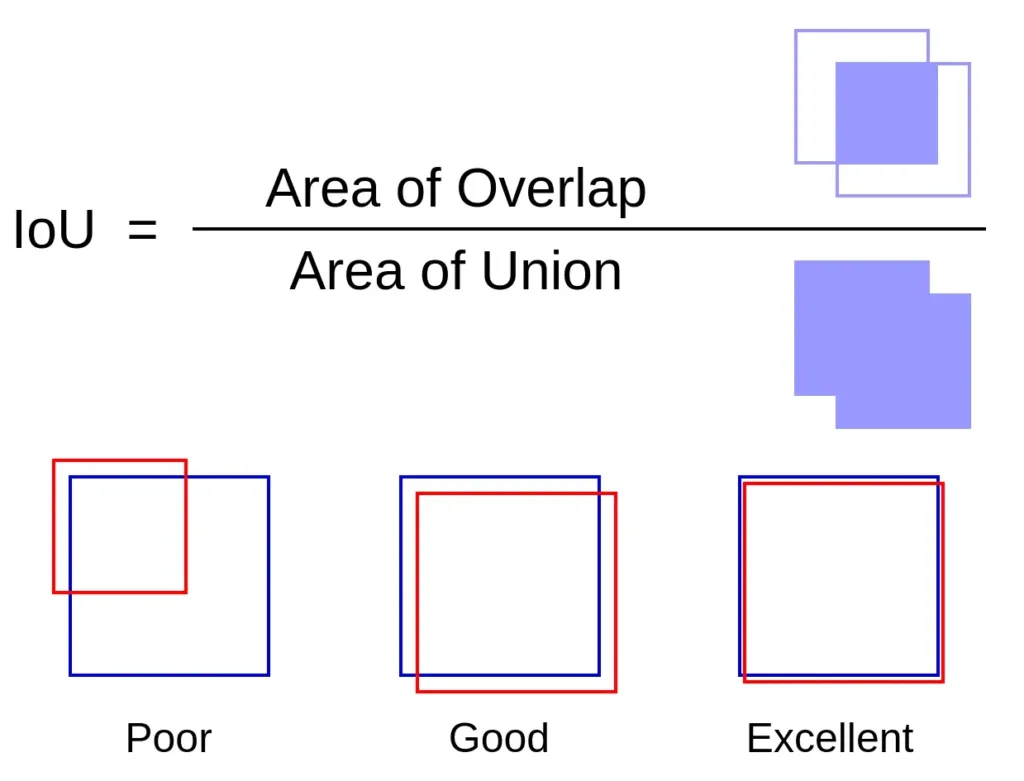
\includegraphics[width=0.5\linewidth]{img/iou.png}
    %\vspace{0.5cm}
    \caption{A diagram representing the Intersection over Union (IoU)}
    \label{metric:iou}
\end{figure}

This metric is crucial in assessing the performance of semantic segmentation models as it provides a quantitative measure of how well the model is able to localize objects within an image. A higher IoU score signifies better localization accuracy and thus, better performance of the detection algorithm.

Furthermore, IoU is often used as a threshold for determining true positives, false positives, and false negatives in object detection tasks, thereby enabling the calculation of other performance metrics such as precision, recall, and F1-score.

% \subsection{Average Precision}
% In the context of image segmentation, Average Precision (AP) remains a crucial performance metric, providing insight into the accuracy of algorithms in segment the object boundaries. Unlike object detection, where bounding boxes are evaluated, segmentation assesses pixel-wise classification, making AP a valuable tool for quantifying segmentation quality on the predicted object mask.

% To compute AP in segmentation, precision and recall are calculated differently compared to object detection. Here, precision measures the ratio of correctly classified pixels (true positives) to the total number of pixels classified as positive (true positives and false positives). Recall, on the other hand, assesses the ratio of correctly classified pixels to the total number of ground truth positive pixels (true positives and false negatives).

% The calculation of AP involves generating a precision-recall curve by varying the segmentation threshold, which determines what constitutes a positive prediction. At each threshold, precision and recall values are computed, and the area under this curve (AUC) represents the AP score. Higher AP values indicate better segmentation performance, capturing both the precision and recall of the segmentation algorithm across different thresholds.

% AP in segmentation is particularly useful for evaluating the ability of algorithms to accurately delineate object boundaries and handle class imbalance within images. It provides a comprehensive assessment of segmentation quality, considering both the accuracy of positive predictions and the ability to capture all relevant objects in the scene.

% When used alongside other segmentation metrics such as Intersection over Union (IOU) or Dice coefficient, AP contributes to a more nuanced understanding of segmentation algorithm performance, helping researchers and practitioners choose the most suitable models for their specific applications.

\section{Watermark Removal}
In this section, we will run experiments on our pipeline. As mentioned in Section \ref{sec:pipeline}, our watermark removal pipeline consists of two main stages: watermark localization and image inpainting. For an image containing a watermark, we first try to identify the location of the watermark, then cover it up and proceed with inpainting using a diffusion model. In the following subsections, we will detail the models and specific methods for each stage, carry out the watermark removal process in these two stages on the dataset mentioned in Section \ref{sec:dataset}. The experimental results and evaluations will also be provided, showing the overall performance of the pipeline on the task of attacking on the watermark.

\label{sec:removal}
\subsection{Watermark Localization}
\subsubsection{Localization methods}
Locating the region to determine where we should attack is a crucial aspect of our proposed pipeline, as we believe it will help improve the results of watermark removal. At this stage, with the watermarked image and its ground truth of the watermark object on the original image as mentioned in Section \ref{sec:embedding}, we will explore methods to localize the watermark's position in the image. This includes identifying information such as the object's boundary, the minimal bounding box of the region containing the watermark, or even using a mask to indicate the watermark's precise location.

\begin{figure}[t]
    \centering
    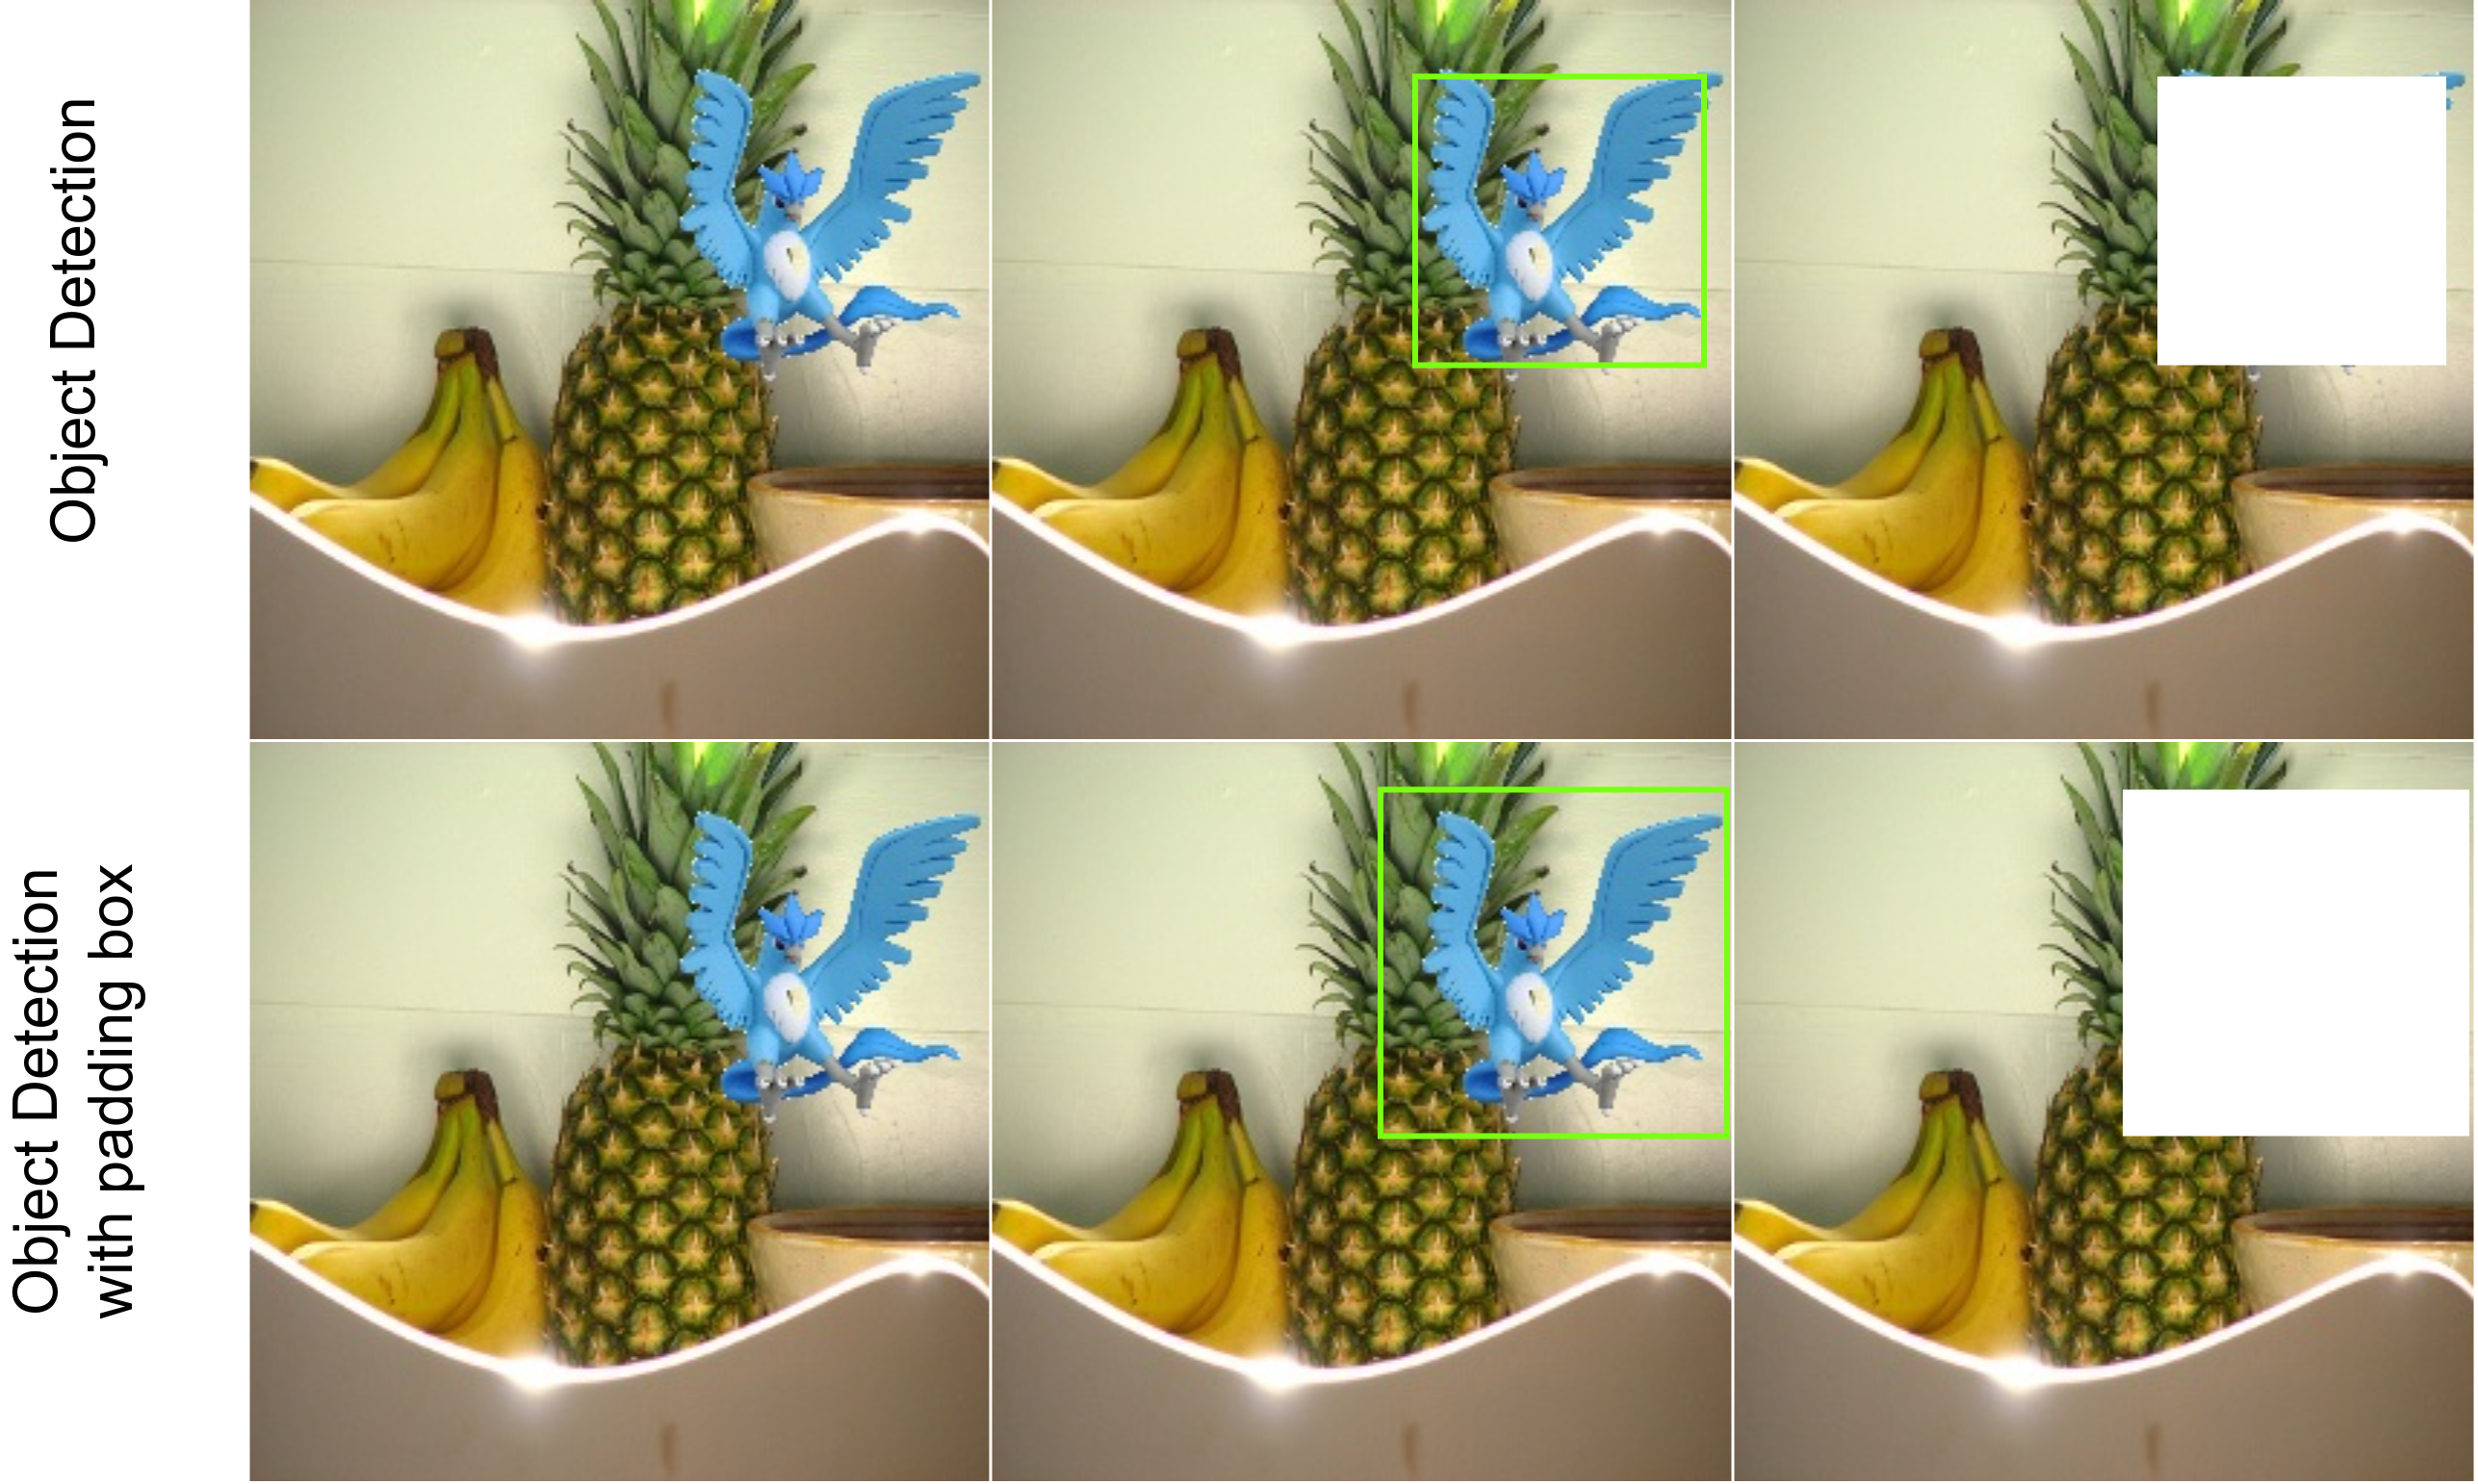
\includegraphics[width=0.8\linewidth]{img/od_w_postprocess.png}
    %\vspace{0.5cm}
    \caption{Localize the watermark with object detection and its post-processing}
    \label{fig:od_w_postprocess}
\end{figure}

There are many ways to localize a watermark in an image. In computer vision and deep learning, we can identify it using models of object detection or segmentation. The object detection method may yield a better result since it only needs to identify the bounding box where the object is, instead of segmentation, which requires per-pixel classification to detect the exact region of the object with a mask. Therefore, applying the object detection method can provide better accuracy and simple post-processing step by adding padding to ensure it covers the entire object as show in Figure \ref{fig:od_w_postprocess}. However, in this pipeline, we decided to use the segmentation method to identify the watermark instead of object detection. The reason for this decision will be illustrated in Figure  \ref{fig:localize-compare-OD-segment}.

\begin{figure}[t]
    \centering
    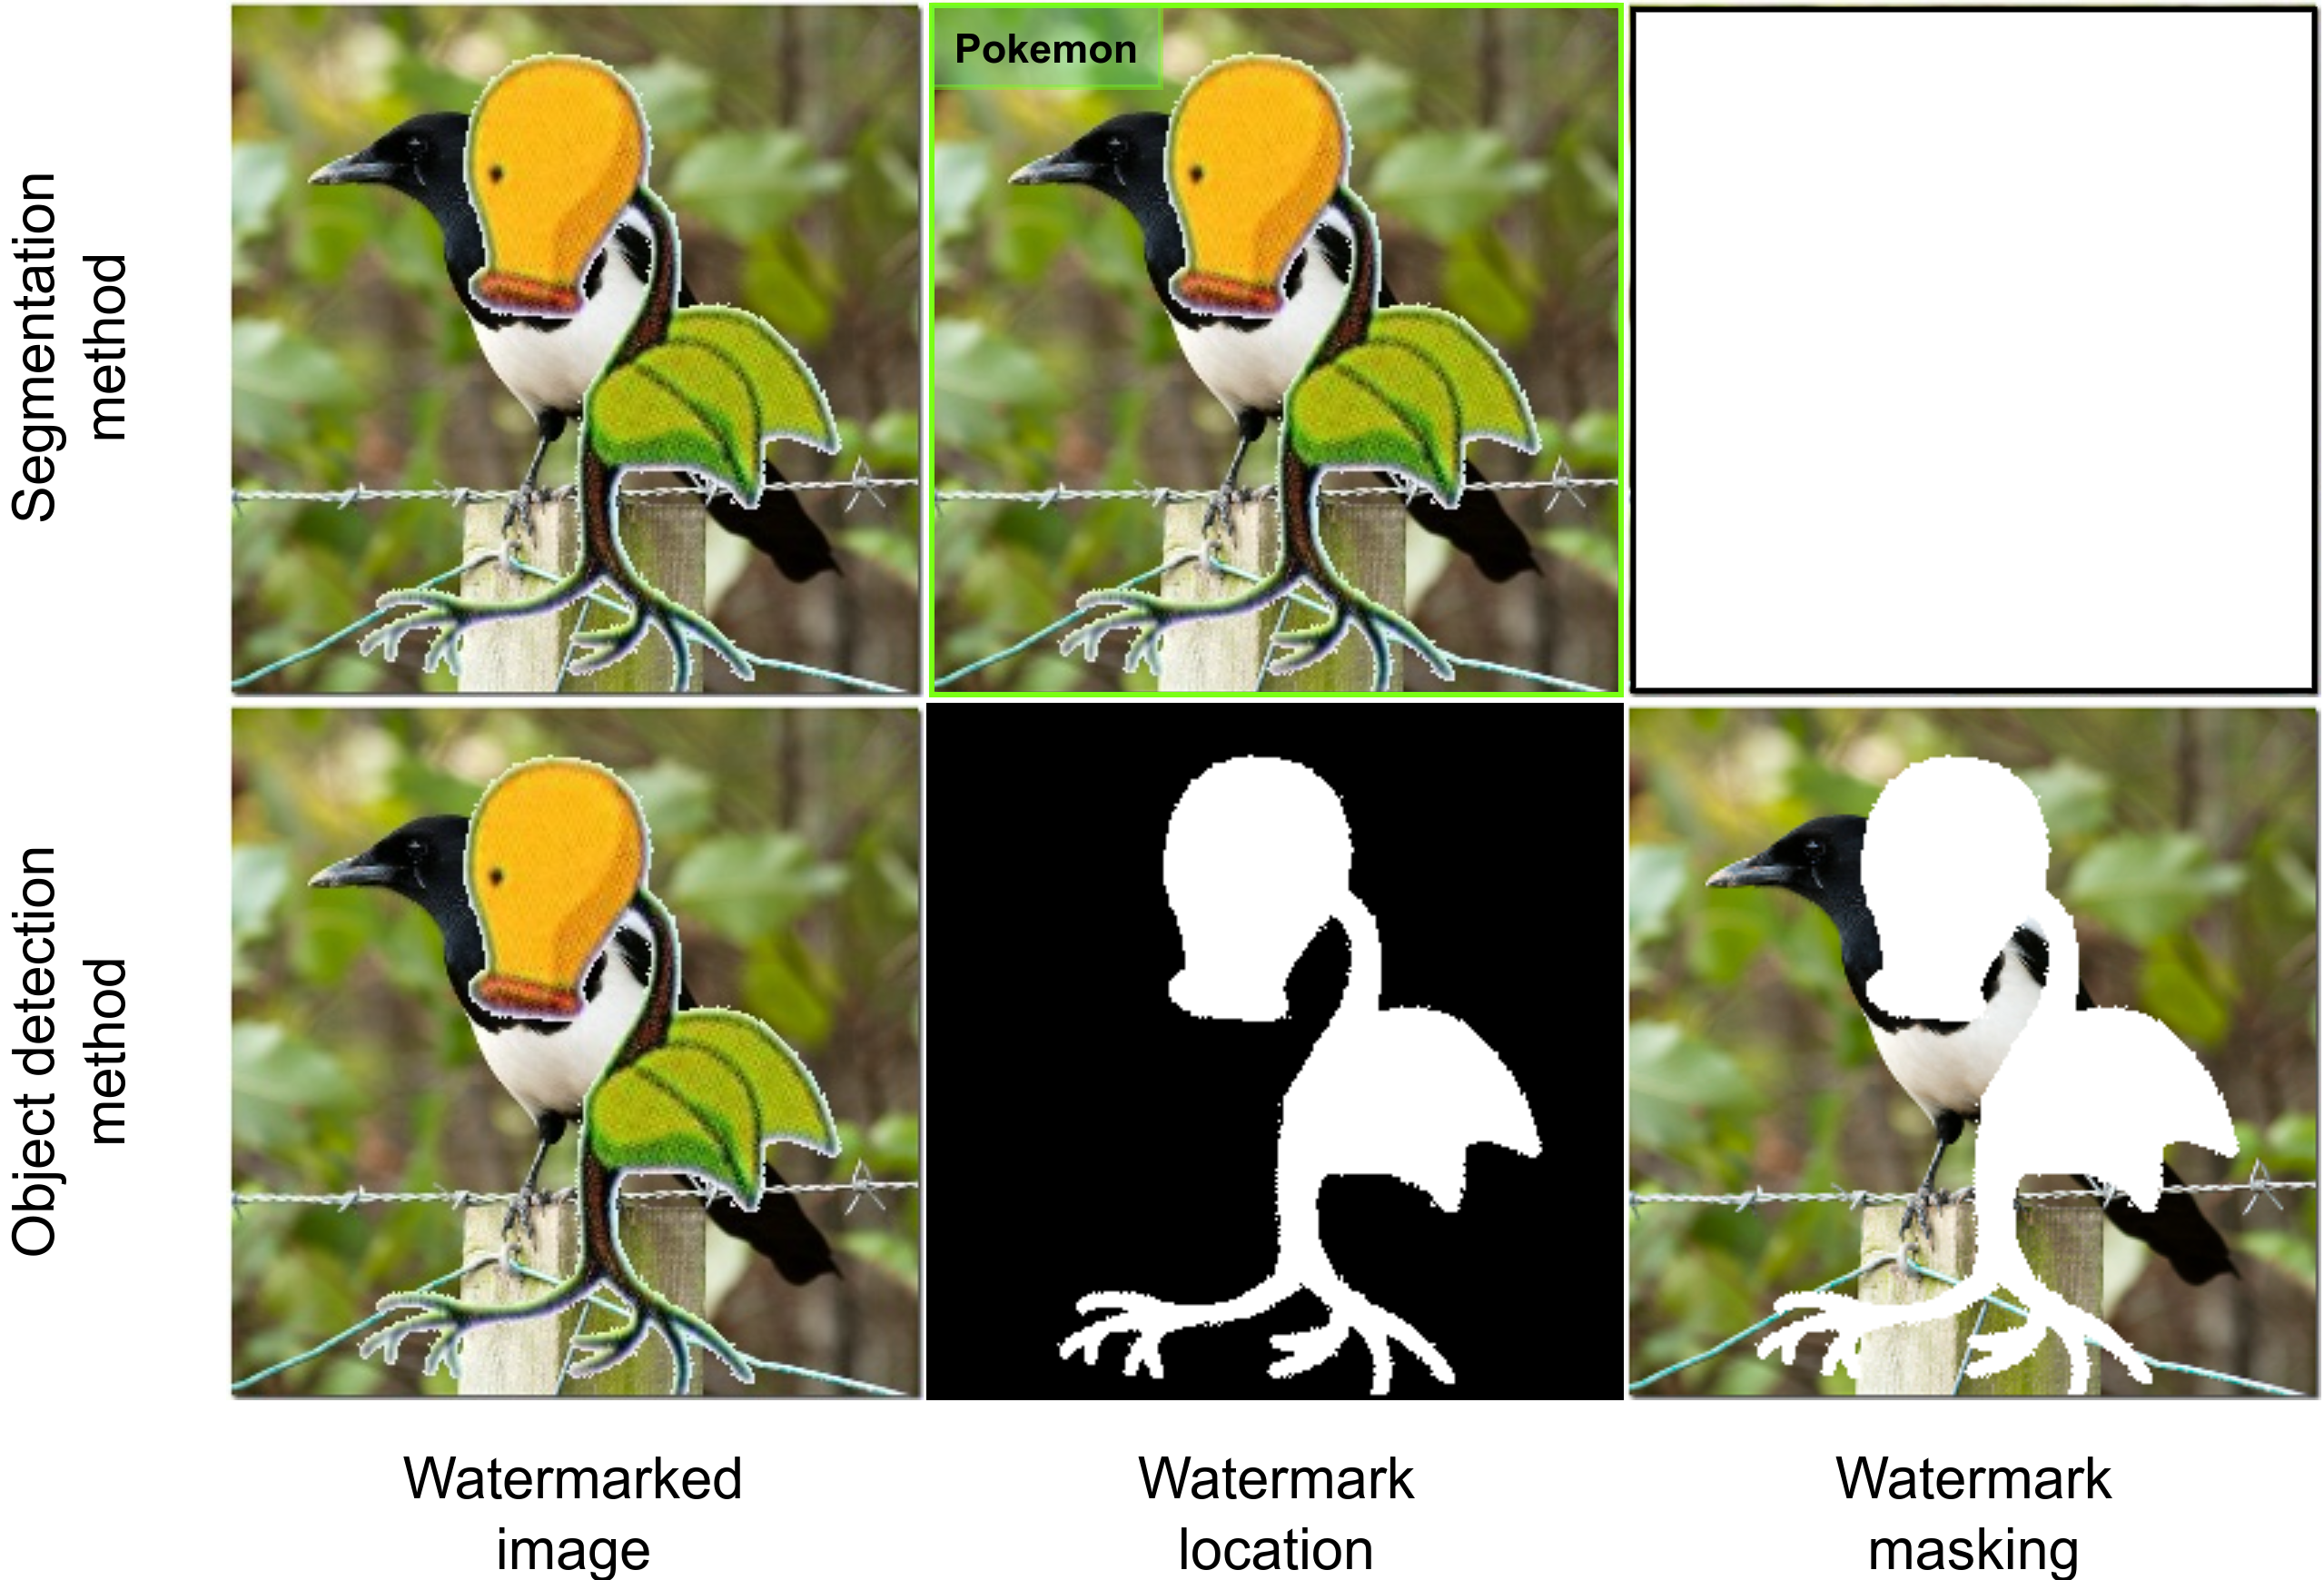
\includegraphics[width=0.8\linewidth]{img/od-segmentation-compare.png}
    %\vspace{0.5cm}
    \caption{Localize the watermark object with object detection and segmentation method}
    \label{fig:localize-compare-OD-segment}
\end{figure}

In Figure \ref{fig:localize-compare-OD-segment}, we can see that the watermark object occupies a large portion of the image. At this point, we can use object detection and semantic segmentation to identify the location of the watermark. In the second column of Figure \ref{fig:localize-compare-OD-segment}, we observe that when using the object detection method, the bounding box of the object occupies almost 100\% of the image area, whereas in reality, the watermark object occupies just over 60\% of the image area. Furthermore, in the next step, after identifying the watermark, we will cover the watermark area and restore the image using image inpainting. With nearly the entire image being covered in this way, performing the next step is completely impractical because there is no information left to be restored, as shown in the last column of Figure \ref{fig:localize-compare-OD-segment}. On the other hand, when using segmentation to identify the location, the watermark object is now identified by a mask that fits the object and occupies exactly the area that the watermark object takes up in the image. This way, we can mask it and reconstruct the image while ensuring that information in the image unrelated to the watermark object is not lost. Hence, we decided to use the segmentation method to localize the watermark object in our pipeline.

\subsubsection{Semantic Segmentation with SegFormer Model}

As mentioned in Section \ref{intro:segformer}, SegFormer \cite{xie2021segformer} is a segmentation model with a transformer-based architecture. The transformer architecture enhances the accuracy of models in computer vision in general and segmentation in particular. Unlike the first segmentation model using transformers, SERT \cite{zheng2021rethinking}, our team chose a lighter model due to resource limitations, but still ensures accuracy in segmentation, which is SegFormer. The performance of the SegFormer and its efficiency will be illustrated in Figure \ref{fig:SegFormer-chart-performance}.

\begin{figure}[t]
    \centering
    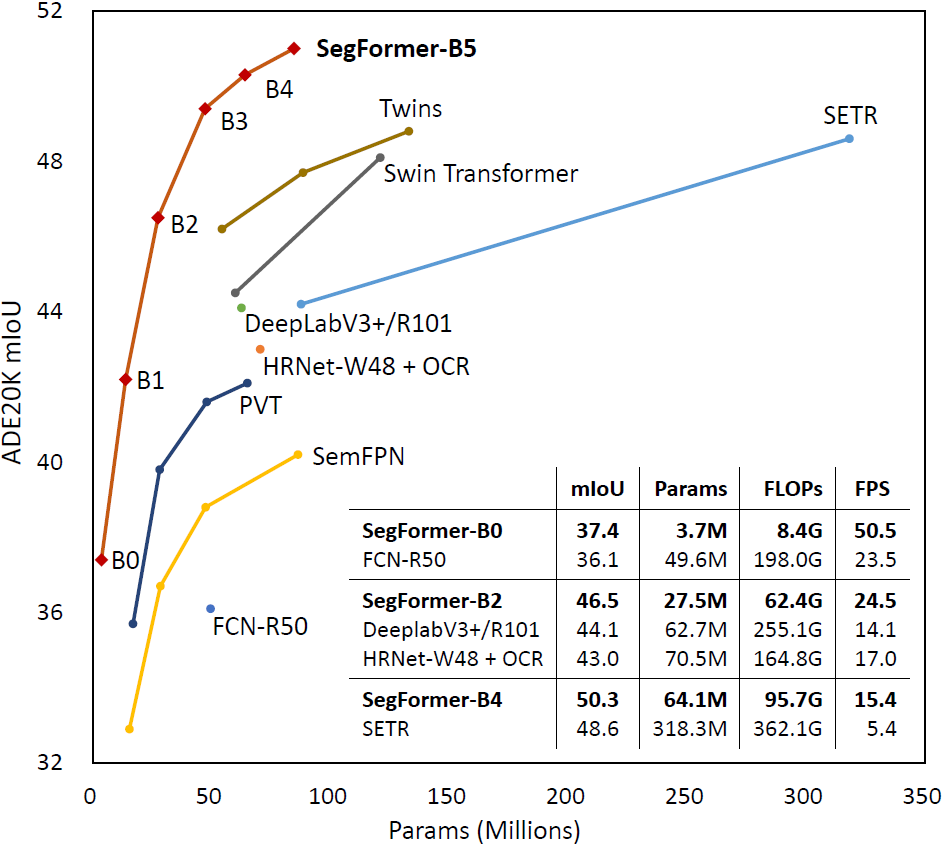
\includegraphics[width=0.5\linewidth]{img/segformer-performance.png}
    %\vspace{0.5cm}
    \caption[SegFormer and other model performance]{SegFormer performance vs. model efficiency on ADE20K dataset compare to other segmentation models \cite{xie2021segformer}}
    \label{fig:SegFormer-chart-performance}
\end{figure}

To train the SegFormer model for watermark localization, we prepared a dataset consisting of approximately 39,000 images containing 50 types of watermarks, with segmentation mask labels of the watermark objects as detailed in Section \ref{sec:embedding}. The model was trained for about 9 hours on an NVIDIA RTX A4500 GPU. After training, we obtained the segmentation results on the validation dataset, which are described in the second row of Figure \ref{fig:segmentation-result}.

\begin{figure}[t]
    \centering
    \includegraphics[width=\linewidth]{img/segmentation-result.png}
    %\vspace{0.5cm}
    \caption[Segmentation result]{Segmentation result when training with SegFormer and Zero-shot inference by prompts with SAM}
    \label{fig:segmentation-result}
\end{figure}

From the results in the second row of Figure \ref{fig:segmentation-result}, we observe that SegFormer yields notable results in segmenting the watermark in the image. The results in the figure show that when we tested the segmentation inference with SegFormer on the validation dataset, the watermark object, which is the Pokémon, was segmented very well from the image. Compared to other methods shown in the figure, SegFormer outperformed them in this validation test by maintaining the consistency of the watermark across various environments of the original image and achieving accurate segmentation from the image. We also evaluated the results using the mIOU metric, which indicates that we achieved 93.22\% on our dataset, demonstrating excellent performance in localizing the watermark in the image.


\subsubsection{Zero-shot Segmentation with Segment Anything Model (SAM)}
The results achieved for localizing watermark objects in images using the SegFormer model are very promising. However, we are interested in exploring a new method. By using an off-the-shelf image inpainting model, we have an idea to investigate a method that can identify watermarks without the need for training. This means that we can run our watermark attacking pipeline without the need to train on a new dataset, also known as a zero-shot pipeline.

After research, we discovered a recent state-of-the-art (SOTA) model that allows us to do just that, called the Segment Anything Model (SAM) developed by Facebook. As mentioned in Section \ref{sec:intro-sam}, the SAM model allows us to segment any object in an image using points or box prompts. Now, we will conduct experiments on this model by preparing prompts using points or boxes and then running the model along with evaluations.

We start with experimenting using a 1-point prompt. We also experimented on our validation dataset with 7500 images and 50 types of watermarks. The 50 types of watermarks are fixed, so we prepare point prompts by identifying a point to select on each watermark object so that the watermark object area when inferred through the SAM model is as complete as possible. Then, combining with the location information of the watermark object in the images we saved, we will determine the points to select for the images so that the model can best segment the watermark area. From what we have prepared, we will inference through SAM and obtain the results in the third row of Figure \ref{fig:segmentation-result}.

From the results  shown in the third row of Figure \ref{fig:segmentation-result}, we can see that by using a 1-point prompt, we can identify the watermark object mask in some cases, such as the first image or the fourth image in the row. However, using a 1-point prompt when inferring with SAM sometimes causes the model to not fully understand what object it needs to identify. For example, in the third or the last image in that row, we can see that SAM considers a large area of surrounding objects as part of the object selected with the 1-point prompt. This can happen due to similarities in color or edges of the objects being adjacent to each other. Moreover, when calculating the accuracy using the mIOU metric for the experiment with the 1-point prompt for SAM, we obtained a result of 75.72\% for using the 1-point prompt to identify the watermark object. While this is not an very impressive score, it demonstrates that this method is feasible for zero-shot segmentation for our watermark dataset. This is because SAM provides better input prompts that we can continue to experiment with and evaluate.

With the results obtained from the 1-point prompt, we realize the potential of SAM in serving as a zero-shot model for our problem. Furthermore, the SAM model allows us to input more than one point for the prompt. Therefore, we continue experimenting by selecting the four best points for each watermark object. Similarly to the 1-point prompt, we have prepared 4-point prompts and inference through SAM on the validation dataset. The results of this experiment are described in the forth row of Figure \ref{fig:segmentation-result}.


From the results shown in the forth row of Figure \ref{fig:segmentation-result}, we can see that now, the objects are segmented much better compared to using only a single point. This is because SAM can be provided with more information related to the object we need to identify in the image, allowing the model to make predictions that closely match the object of interest. By using a 4-point prompt, from the inference test images we obtained, we can see that the watermark object is fully segmented and the likelihood of including surrounding objects is minimized. Moreover, in the fifth image in the row, we can see that the Pokémon shaped like a tree is segmented by SAM even better than by SegFormer, despite the trunk's color being similar to the background, which could potentially cause confusion in the model. Based on the very promising results observed in the inference images, we proceeded to evaluate SAM with a 4-point input prompt on the same validation dataset. The results were extremely impressive, with the mIOU score of SAM with a 4-point prompt being 91.56\%, a very high accuracy rate, especially considering that the model had never seen any training data before.

Using the 4-point prompt yields extremely good results, and we are truly impressed with a zero-shot model, a model that can segment even without being trained on our dataset. Additionally, SAM also supports inputting bounding boxes as prompt, and from there, the model will predict the object to segment in that box region. Therefore, we will utilize the bounding box information prepared in Section \ref{sec:embedding} to use it as input prompt for SAM. By using this method, we obtain the results shown in the last row of Figure \ref{fig:segmentation-result}.

From the results shown in the last row of Figure \ref{fig:segmentation-result}, we can see that by using a bounding box, we can limit the model's observation area and help SAM segment the desired object more easily than by examining the entire image. The results show that using a box prompt also yields better results compared to using a 1-point prompt. Moreover, when watermark objects are confined by a bounding box, the model seems to better understand the differences between the watermark object and other objects in the image, allowing SAM to segment the watermark more clearly than when using a 1-point prompt, which results in a segmentation mask that covers both the watermark and other objects. The evaluation results of the box prompt when running experiments on the validation set showed an mIOU metric of 86.61\%. Although this result is not as good as the 4-point prompt, it opens up a new direction where we can combine object detection and segmentation models to create a higher accuracy zero-shot model in the future.

Finally, we have compiled all the results and evaluations of the segmentation models after experimenting and evaluating on our validation dataset of 7500 images in Table \ref{table:segmentation-result}. From this result table, we can see that using SegFormer for the task of watermark localization in images yields the best result with an mIOU evaluation of 93.22\%. Following that, using SAM with 4-points prompt produces unexpected results of 91.56\%, which is quite good compared to SegFormer even though this is a zero-shot model that has never seen any data before. With the results from this table, we can conclude that using SegFormer is suitable for known watermarks, where we have data to train on and it yields the best results. On the other hand, for unseen watermarks, using SAM is entirely reasonable as it produces very good results, only lagging behind SegFormer by about 2.3\% in mIOU evaluation but without the need for retraining.

\begin{table}[t]
\centering
\begin{tabular}{ll}
\hline
\multicolumn{1}{c}{\textbf{Method}} & \multicolumn{1}{c}{\textbf{mIOU↑}} \\ \hline
\textbf{SegFormer}                             & \textbf{93.22}                                                        \\
SAM with one point                    & 75.72                                                        \\
SAM with four point                   & 91.56                                                        \\
SAM with bounding box                 & 86.61                                                        \\ \hline
\end{tabular}
\caption{Semantic Segmentation evaluation of different methods}
\label{table:segmentation-result}
\end{table}

% \textcolor{red}{Identification -> Localization, change in chart pipeline}

% \textcolor{blue}{
%     In the previous section (Section \ref{sec:ewi}), we have embedded watermarks into images by using image processing method. Then, we need to develop ways to identify them in the watermarked image. In this section, we alleviate the models of segmentation to address this problem.
%     \\
%     1. What is localization. 
%     \\
%     2. There are many ways to identify the watermark in image. In computer vision and deep learning, we can identify it by using models of object detection and segmentation. However, in this pipeline, we decide to use the segmentation method to identify the watermark instead of object detection. The reason will be illustrated in Figure <a figure>
%     \\
%     <Insert some figure here>
%     \\
%     3. From this figure, we can observe that by using object detection, the watermark will be detected at full of this image...\\
%     4. First, we present our result of segmentation when using a transformer-based model, which call SegFormer, that we have introduce in Section...\\
%     5. By using SegFormer, we have archive a notable result on segmentation the watermark in the image, the result is shown in Table ... \\
%     6. However, by using the off-the-shell image inpainting model, we have an idea to make our pipeline is training-free, which mean that we are able to run our watermark attacking pipeline without training on new data, or we also called a zero-shot pipeline. We are going to make it possible by using the recently SOTA zero-shot model, Segment Anything developed by Facebook. 
% }



\subsection{Image Inpainting}
In this section, we will conduct experiments on the inpainting task using the I$^2$SB model. We will perform experiments for the image inpainting task on both the ImageNet dataset, which is a pretrained dataset for I$^2$SB, and other data that we collected, which differ from the original training dataset. Through these experiments, we obtained several results, which are presented below.

\subsubsection{Image Inpainting with ImageNet}
First, we will conduct experiments using the I$^2$SB model on the ImageNet dataset. We will utilize the ground-truth watermark mask extracted in Section \ref{sec:embedding} to create a corrupted image by applying this mask. Subsequently, we will forward the corrupted image through the I$^2$SB model for reconstruction. The results obtained will be described in Figure \ref{fig:i2sb-imagenet-result}.

From Figure \ref{fig:i2sb-imagenet-result}, we can observe that in the first two columns of results, the reconstructed images are very well-done and closely resemble the original images. Particularly in the second column, where the leaf is partially obscured with intricate patterns, and the corrupted image has almost completely covered the leaf, our model has reconstructed it remarkably well, almost identical to the original image. However, it is reasonable that image inpainting might produce some details different from those in the original image; even when looking at a corrupted image, we can only guess what details might lie beneath that mask without being certain until we see a clean image. This is evident in the third and fourth columns. In these images, the patterns on the body of the leopard and the face of the dog have been reconstructed. If we had not seen the clean image, we could see that the model can understand what it needs to draw and is doing a good job of reconstructing the image with many details obscured in the corrupt image.

Moving to the last two columns of results, we can see that the masks have now covered the face of the dog and the chemical flask. In the reconstructed image of the dog, we can see that details such as the teeth or the nose hole have changed slightly, but the expression of the dog remains cheerful like in the original image. In terms of detail, the model is producing an image with many details changed because they were obscured, but the details it guesses are quite reasonable and fit well with the context of the image. In the last image, a chemical flask with a text label is reconstructed. At this point, the model has restored the shape of the flask quite intact and well, but the text on the flask has been altered and is no longer readable. For an inpainting model, guessing what is under the mask with text is extremely difficult, but the fact that they understand there are characters beneath the mask and can reconstruct them is quite promising and lays the foundation for handling text in the future.

\begin{figure}[t]
    \centering
    \includegraphics[width=0.8\linewidth]{img/i2sb-imagenet-result.png}
    %\vspace{0.5cm}
    \caption[Image Inpaiting using I$^2$SB model with ImageNet dataset]{Image Inpaiting using I$^2$SB model with ImageNet dataset}
    \label{fig:i2sb-imagenet-result}
\end{figure}
It is impressive to see such high scores on both PSNR and SSIM metrics, indicating excellent performance in image reconstruction. PSNR of 30.2 falls within the range considered good (30-40), and an SSIM score of 0.96 indicates extremely high structural similarity between the reconstructed and original images. These results demonstrate the effectiveness of the I$^2$SB model in reconstructing images, even in cases where significant portions of the image are missing or corrupted.
\subsubsection{Image Inpainting with other dataset}
After running experiments for the image inpainting part using I$^2$SB on the pre-trained ImageNet dataset, we will continue to perform experiments by running this model with datasets outside the training data. As mentioned in Section \ref{sec:i2sb}, the I$^2$SB model has the ability to reconstruct images with part of the information not masked instead of starting from Gaussian noise like other diffusion-based models. This enables the model to run completely on data outside our trained data. Indeed, when collecting data outside the training data, we tried running the I$^2$SB model with watermark object masks and obtained the results described in Figure \ref{fig:i2sb-difference-dataset-result}.

\begin{figure}[t]
    \centering
    \includegraphics[width=0.8\linewidth]{img/i2sb-difference-dataset-result.png}
    %\vspace{0.5cm}
    \caption[Image Inpaiting using I$^2$SB model with random dataset]{Image Inpaiting using I$^2$SB model other dataset}
    \label{fig:i2sb-difference-dataset-result}
\end{figure}

From the results shown in Figure \ref{fig:i2sb-difference-dataset-result}, we can see that the results obtained from the images outside the training dataset are indeed promising. Despite differences in detail, the model successfully reconstructs parts of the images that were covered or missing, even though they were not present in the training set. This demonstrates the generalization capability of the I$^2$SB model, allowing it to be applied to various datasets without the need for retraining. Furthermore, there is potential for further improvement through additional processing techniques or model tuning to enhance results on more diverse datasets without the need for retraining.

\subsection{Watermark Removal Pipeline}
In this section, after building the watermark localization model and the image inpainting model with a mask, we will complete our two-stage pipeline for watermark removal. At the same time, we will observe, evaluate, and compare the results of watermark removal on our pipeline with other methods.
\subsubsection{CNN-based method}

Recently, while researching models related to the watermark removal problem, we came across a paper called SWCNN \cite{2024swcnn}. This paper was published in 2024 and submitted to the CVPR conference. The paper designs a CNN-based model for the watermark removal task, and it claims to achieve state-of-the-art (SOTA) results compared to previous papers, even outperforming a method using generative models like GAN. The reported results are based on the evaluation table provided by the paper, presented in Table \ref{table:swcnn}.

\begin{table}[t]
    \centering
    \begin{tabular}{cccll}
        \hline
        \textbf{Methods}                             & \textbf{PSNR ↑}  & \textbf{SSIM ↑} \\ \hline
        FFDNet  \cite{zhang2018ffdnet}               & 27.8820          & 0.8778          \\
        DIP  \cite{ulyanov2018deep}                  & 29.7473          & 0.9260          \\
        WGAN-GP  \cite{yu2018generative}             & 31.0752          & 0.9662          \\
        DnCNN  \cite{zhang2017beyond}                & 30.1071          & 0.9620          \\
        {DRD-Net \cite{deng2019drd}}                 & 28.9090          & 0.9707          \\
        {FastDerainNet \cite{wang2020fastderainnet}} & 32.2593          & 0.9815          \\
        {EAFNWDD \cite{sun2021efficient}}            & 33.4744          & 0.9700          \\
        \textbf{SWCNN} \cite{2024swcnn}              & \textbf{36.9022} & \textbf{0.9893} \\ \hline
    \end{tabular}
    \caption[Watermark removal performance of different methods]{Watermark removal performance of different methods\cite{2024swcnn}}
    \label{table:swcnn}
\end{table}

From there, we set up to train this model on our dataset. We prepared the same training and validation dataset, along with the 50 types of watermarks used for evaluating our pipeline. After training for 5 hours, we obtained the results of this model. The performance of the model when trained and tested on our dataset is approximately 25.64 on the PSNR metric and 0.85 on the SSIM metric. The results are summarized in Table \ref{table:swcnn}.

\subsubsection{Our Pipeline with Segmentation and Image Inpainting}

After preparing the necessary models, we finally combined them and started running our pipeline. Firstly, for Watermark Localization, we performed inference and observed that although the SegFormer model had been trained and produced very good results, there were still some errors in the segmentation mask results, as shown in Figure \ref{fig:segformer-no-dilate}.

\begin{figure}[t]
    \centering
    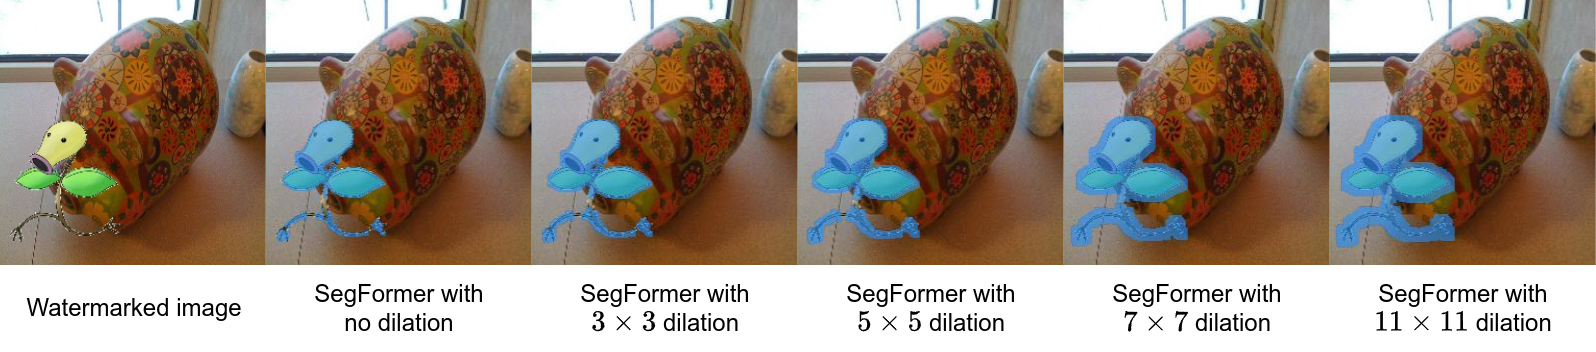
\includegraphics[width=\linewidth]{img/dilation-segformer.png}
    %\vspace{0.5cm}
    \caption[SegFormer Segmentation post-processing]{SegFormer Segmentation result with inaccurate mask and post-processing by different dilation kernel}
    \label{fig:segformer-no-dilate}
\end{figure}

From Figure \ref{fig:segformer-no-dilate}, we can see that the resulting segmentation mask may still have some shortcomings, especially in cases where the watermark object has a color similar to objects in the image. To address this, we experimented with a post-processing method called dilation. Dilation is a technique that extends the segmentation mask, allowing erroneous parts of the mask to be connected, thus helping to fully encompass the object in a single mask. However, when applying the dilation method, we need to select the kernel size carefully, as different kernel sizes will yield different results. We conducted experiments to select an appropriate kernel size, and the results are shown in Table \ref{fig:segformer-no-dilate} and Figure \ref{fig:segformer-no-dilate}.

From the experimental results on various dilation kernels, we can see that if we use small kernels like $3 \times 3$ or $5 \times 5$, the continuity of the segmentation mask is still not fully improved. With the use of a $7 \times 7$ kernel, our segmentation mask has been completely connected and can greatly improve the results. With larger kernel sizes, as we can observe in Table \ref{fig:segformer-no-dilate} and Figure \ref{fig:segformer-no-dilate}, using a larger kernel than necessary will inflate our segmentation mask, causing the image inpainting model to predict on a larger mask, thereby reducing the model's evaluation metrics.

\begin{table}[t]
    \centering
    \begin{tabular}{lll}
        \hline
        \multicolumn{1}{c}{\textbf{Method}}                                                & \multicolumn{1}{c}{\textbf{PSNR ↑}} & \multicolumn{1}{c}{\textbf{SSIM ↑}} \\ \hline
        SegFormer + I$^2$SB & 25.13                                & 0.87                                 \\ 
        SegFormer + I$^2$SB + ($3 \times 3$) dilation & {25.81}                       & {0.88}                        \\ 
        SegFormer + I$^2$SB + ($5 \times 5$) dilation & {25.82}                       & {0.88}                        \\ 
        SegFormer + I$^2$SB + ${(7 \times 7)}$ {dilation} & \textbf{27.82}                       & \textbf{0.90}                        \\ 
        SegFormer + I$^2$SB + ($11 \times 11$) dilation & {26.82}                       & {0.89}                        \\ \hline
    \end{tabular}
    \caption{Segmentation post-processing performance with different settings}
    \label{table:segformer-kernel}
\end{table}
With the experimentation of dilation post-processing for the segmentation mask as previously conducted, we will now proceed with the watermark removal pipeline by applying dilation with a kernel size of $7 \times 7$ to ensure the accuracy of the segmentation mask. The results obtained from our pipeline are summarized in Table \ref{table:wtm-rmv}. From this table, we can observe that the combination of SegFormer and I$^2$SB for our pipeline is yielding the best results in terms of PSNR evaluation with a score of 27.82 along with a metric score of 0.90 for SSIM. This result is highly impressive as it closely approaches the results of using I$^2$SB on the ImageNet dataset. Moreover, this result outperforms the results of SWCNN, a paper that claims to produce the best results for watermark removal and has beaten several GAN models for this task. Furthermore, another notable result is the combination of SAM with a 4-point prompt and I$^2$SB also yields extremely high results, even the best on the SSIM metric with a score of 0.91. This is noteworthy as the combination of SAM and I$^2$SB is an idea for a Zero-shot pipeline, where we can use a watermark removal pipeline without the need to retrain on new data.
\begin{table}[!t]
    \centering
    \begin{tabular}{lll}
        \hline
        \multicolumn{1}{c}{\textbf{Method}}                                                & \multicolumn{1}{c}{\textbf{PSNR ↑}} & \multicolumn{1}{c}{\textbf{SSIM ↑}} \\ \hline
        Labeled mask + I$^2$SB    & \textbf{30.2}                        & \textbf{0.96}                        \\ \hline
        SWCNN  \cite{2024swcnn}                                                                             & 25.64                                & 0.85                                 \\  \hline
        SegFormer + I$^2$SB & 25.13                                & 0.87                                 \\ 
        SegFormer + I$^2$SB + dilation & \textbf{27.82}                       & {0.90}                        \\ \hline
        SAM with 1 point + I$^2$SB + dilation  & {21.71}                       & {0.80}                        \\
        SAM with 4 points + I$^2$SB + dilation  & {25.92}                       & \textbf{0.91}                        \\ 
        SAM with boxes + I$^2$SB + dilation & {24.76}                       & {0.89}                        \\ \hline
    \end{tabular}
    \caption{Watermark removal performance of different methods}
    \label{table:wtm-rmv}
\end{table}

% \textcolor{red}{- Bỏ center mask đi, dùng phần random mask rồi viết lại phần kết quả của chạy riêng I2SB cho labeled mask
% \\
% - Nhắc lại phần identify watermark -> kết quả của segformer w/o dilation
% \\
% - Nói về việc Dialate mask (dùng kernel 7x7 qua 1 vòng dilate) để mở rộng phần xác định wtm -> ra kết quả tốt hơn
% \\
% - Giải thích thêm về chọn kernel dialate và list kết quả trên các kernel khác (3x3, 5x5, 9x9, 11x11)
% \\
% - Thử xem lại loss segmentation để lập luận cách xác định kích thước kernel dilation
% \\
% - Các kết quả của data mình trong các related work
% \\
% - SCOPE: Tập trung xử lý ảnh -> xử lý visible watermark}


% \section{Write for DEMO}